\begin{figure*}[t]
	\begin{small}
		\centering
		\vspace{-5mm}
		%    \begin{footnotesize}
		\begin{tabular}{cccc}
			%\multicolumn{4}{c}{\hspace{-4mm} \includegraphics[height=5mm]{./Figs/legend_large.eps}} \vspace{-1mm} \\
			\hspace{-4mm} 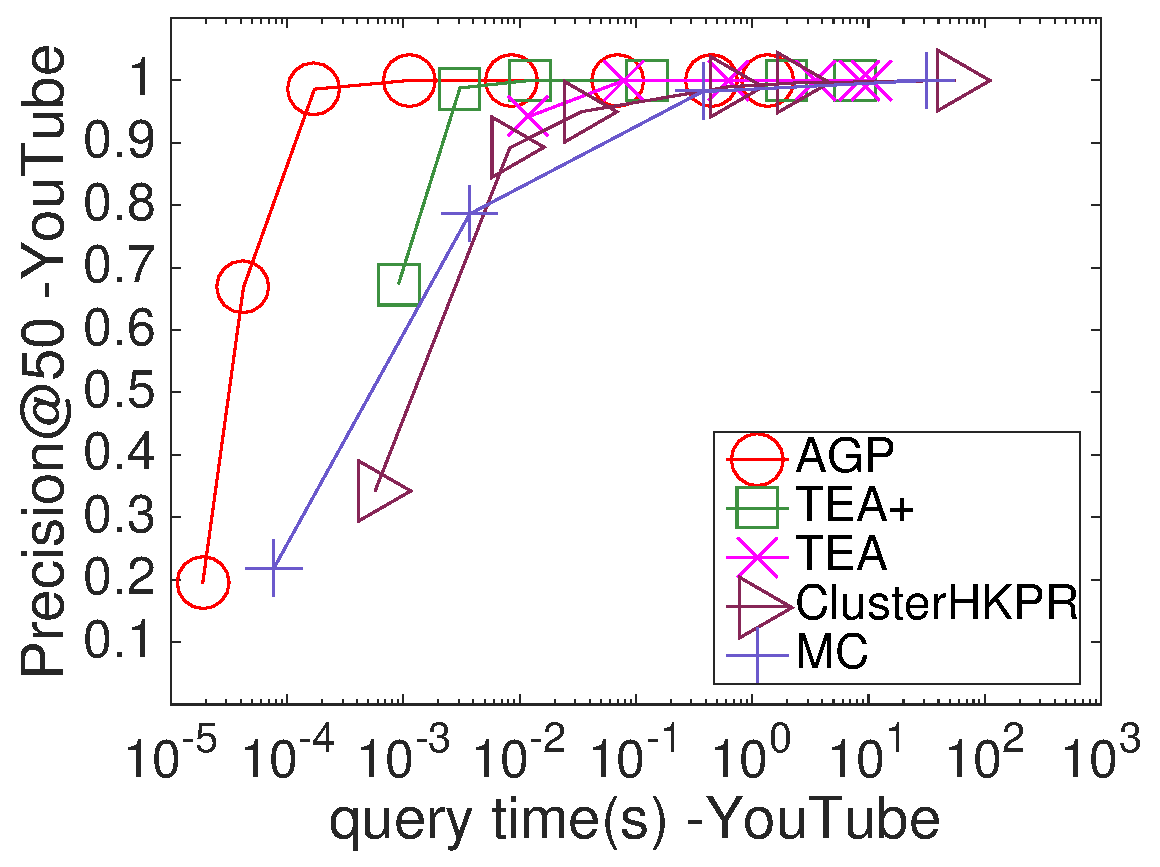
\includegraphics[height=32.7mm]{./Figs/HKPR-precision-query-YT.eps} &
			%\hspace{-3mm} 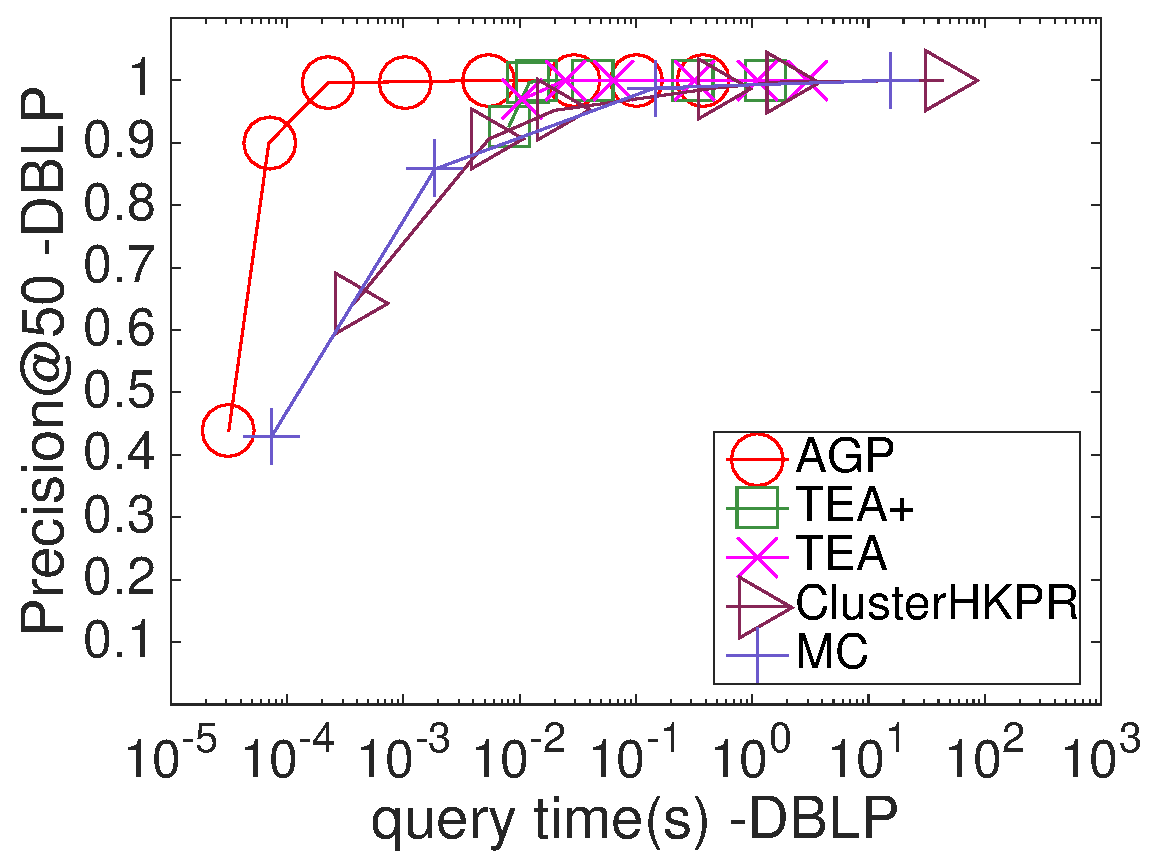
\includegraphics[height=25mm]{./Figs/HKPR-precision-query-DB.eps} &
			\hspace{-4mm} 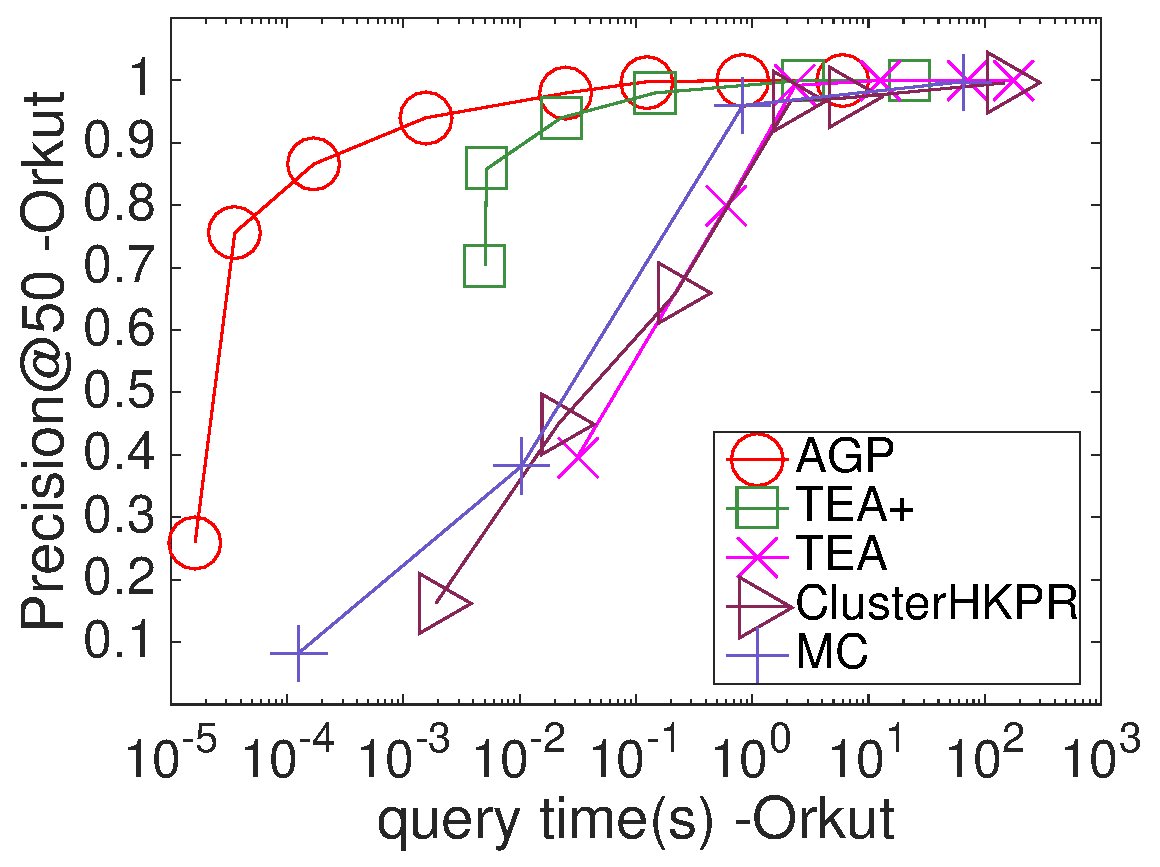
\includegraphics[height=32.7mm]{./Figs/HKPR-precision-query-OL.eps} &
			\hspace{-4mm} 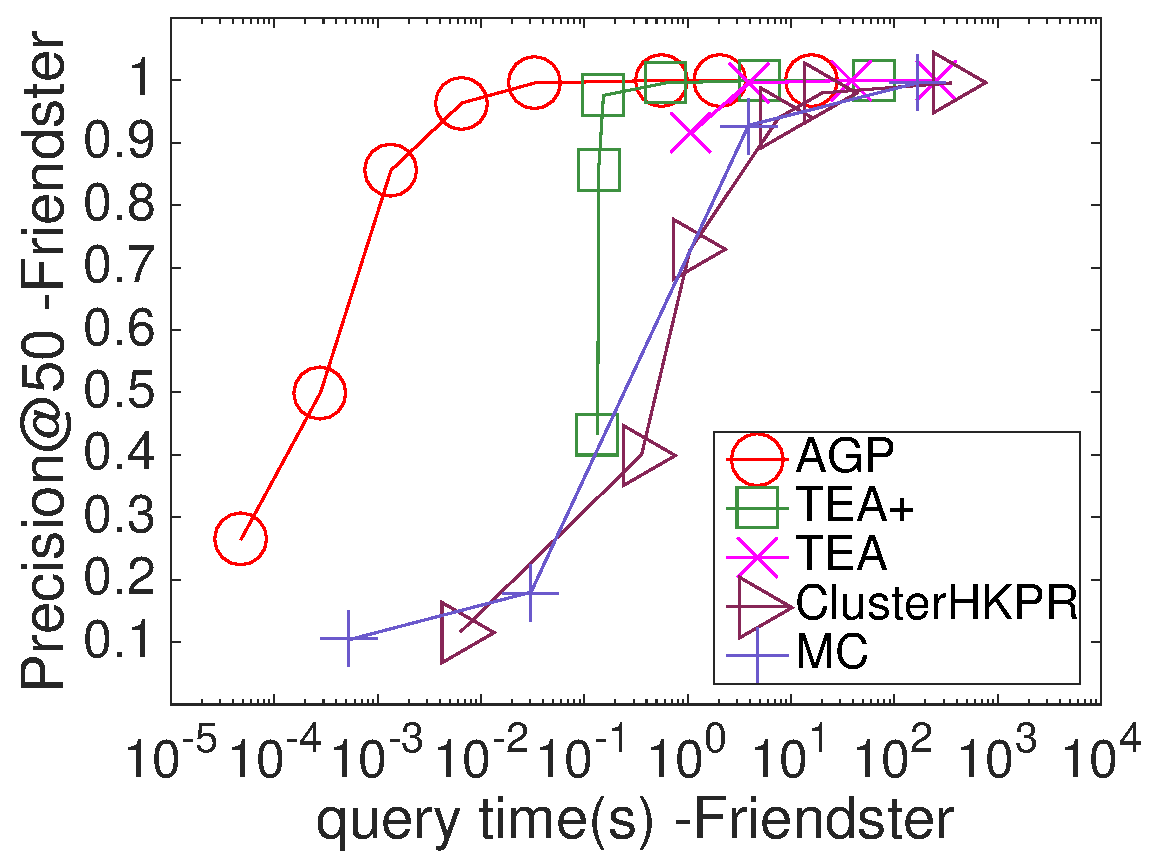
\includegraphics[height=32.7mm]{./Figs/HKPR-precision-query-FR.eps} &
			\hspace{-4mm} 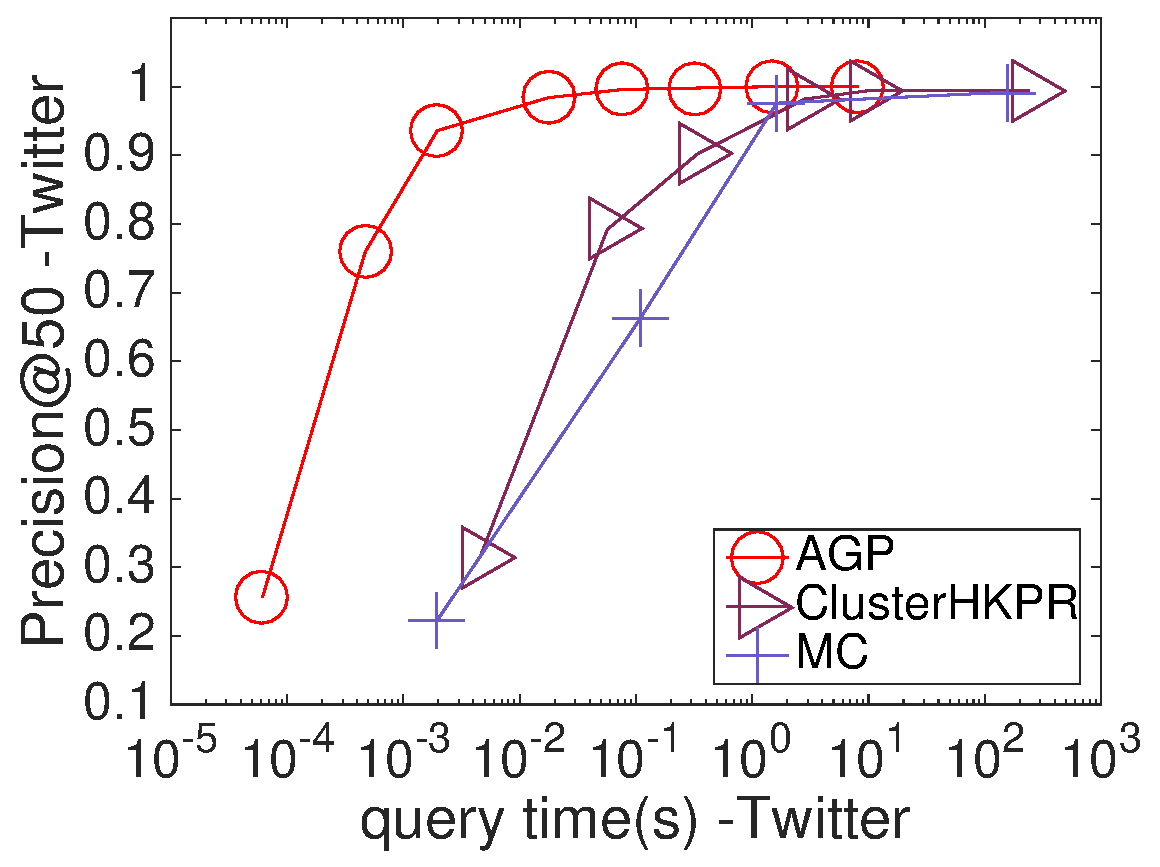
\includegraphics[height=32.7mm]{./Figs/HKPR-precision-query-TW.eps} 
		\end{tabular}
		\vspace{-5mm}
		\caption{Tradeoffs between {\em Normalized Precision@50} and query time in local clustering.}
		\label{fig:HKPR-precision-query}
		%\vspace{-2mm}
	\end{small}
\end{figure*}


\begin{figure*}[t]
	\begin{small}
		\centering
		\vspace{-1mm}
		%    \begin{footnotesize}
		\begin{tabular}{cccc}
			%\multicolumn{4}{c}{\hspace{-4mm} \includegraphics[height=5mm]{./Figs/legend_large.eps}} \vspace{-1mm} \\
			\hspace{-4mm} 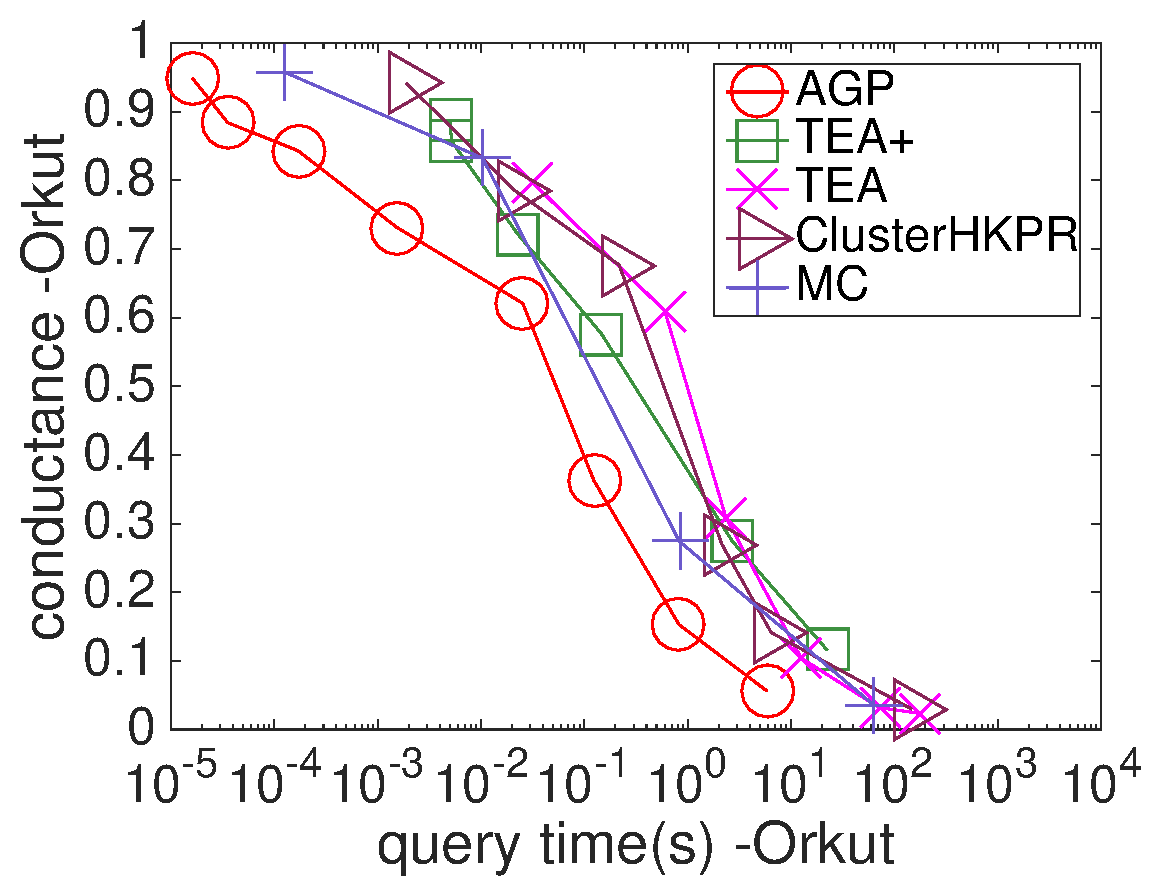
\includegraphics[height=34mm]{./Figs/HKPR-conductance-query-OL.eps} &
			\hspace{-4mm} 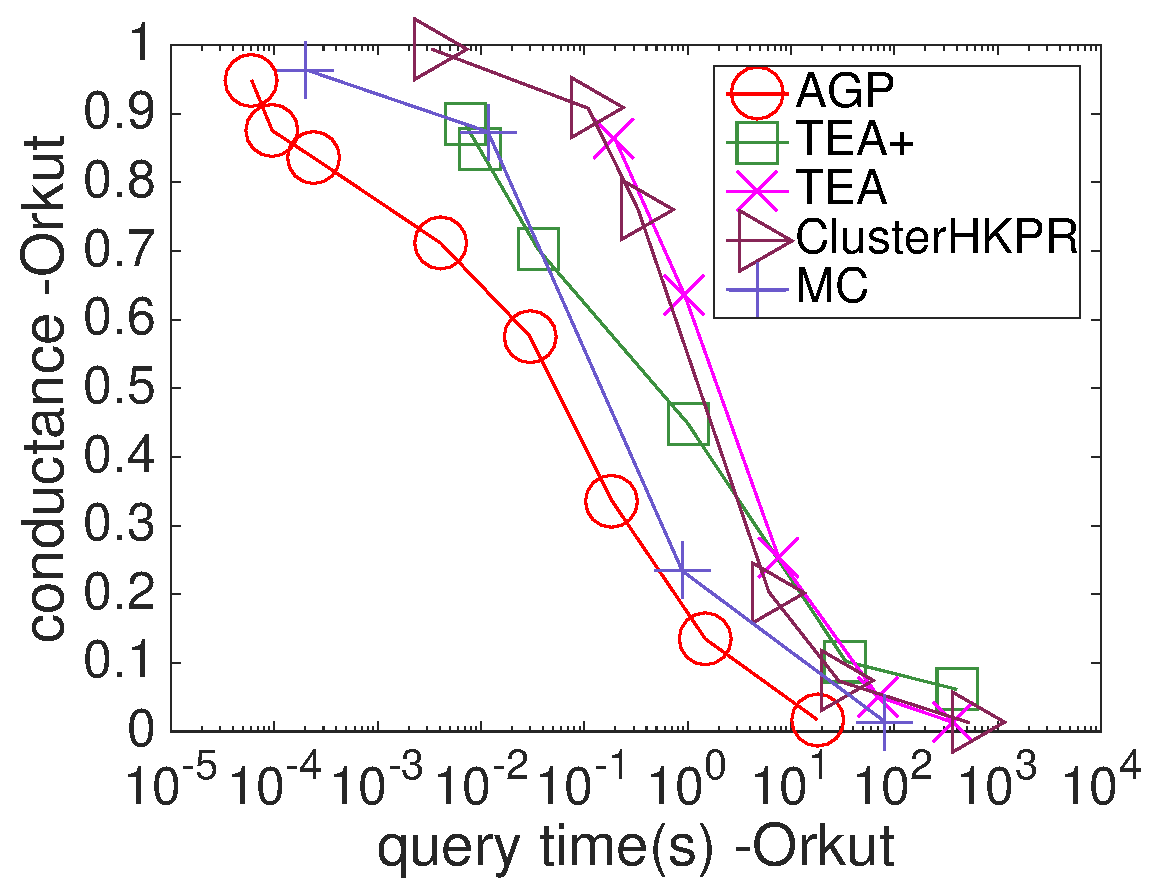
\includegraphics[height=34mm]{./Figs/HKPR-10-conductance-query-OL.eps} &
			\hspace{-4mm} 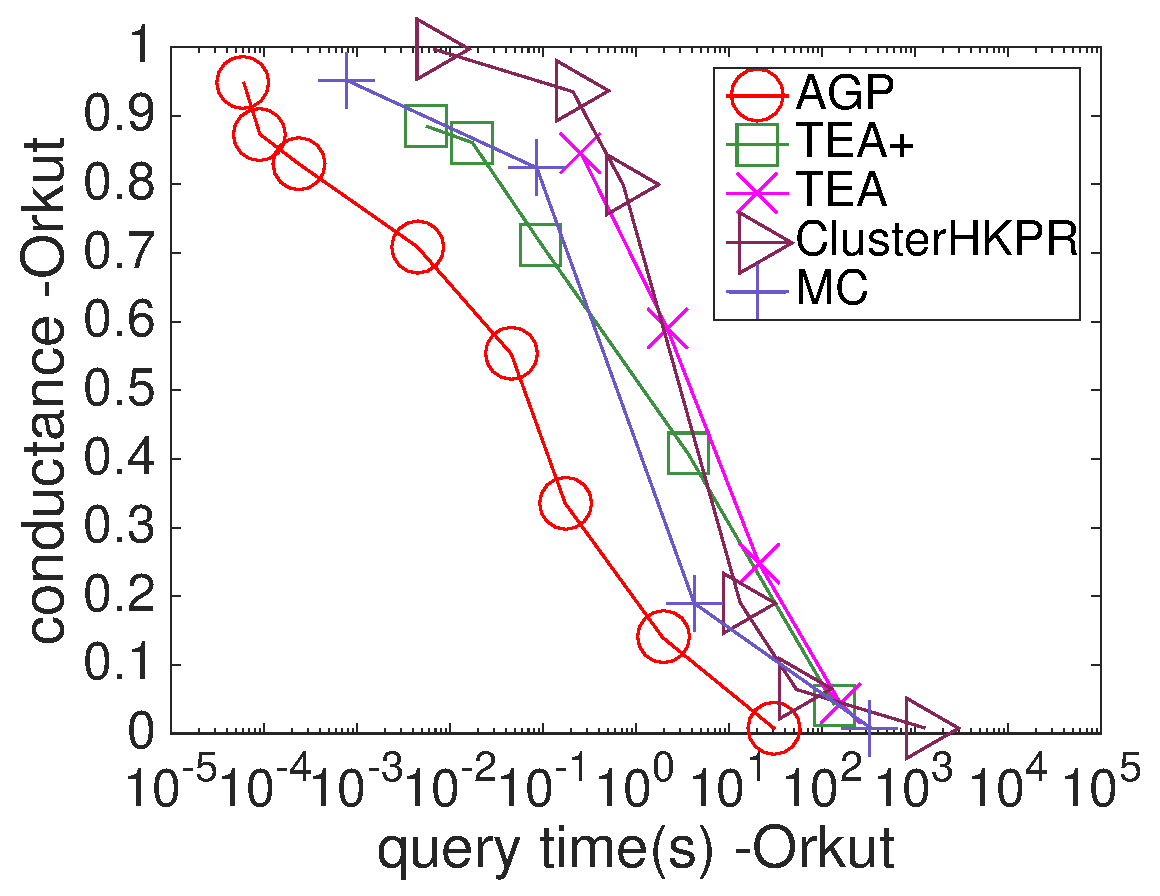
\includegraphics[height=34mm]{./Figs/HKPR-20-conductance-query-OL.eps} &
			\hspace{-4mm} 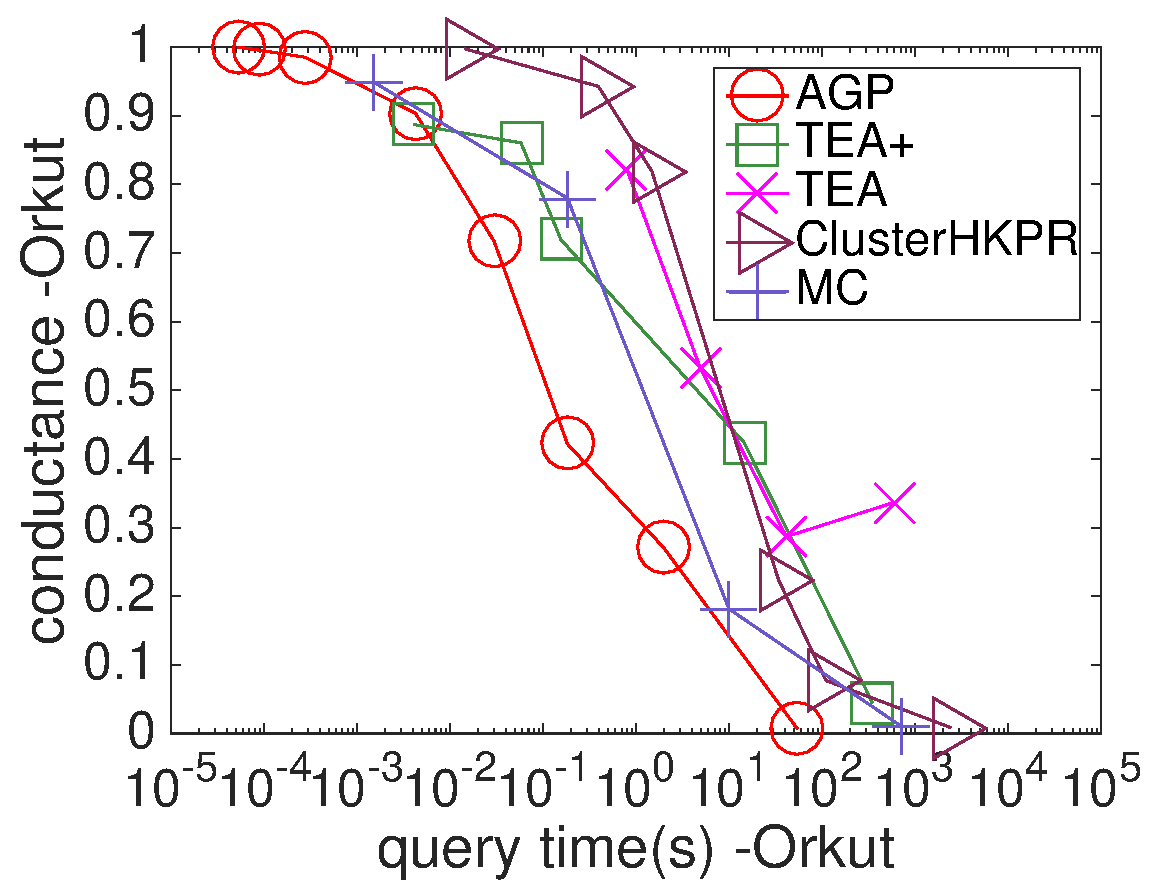
\includegraphics[height=34mm]{./Figs/HKPR-40-conductance-query-OL.eps} \\
			(a) $t=5$ & (b) $t=10$ & (c) $t=20$ & (d) $t=40$ 
		\end{tabular}
		\vspace{-5mm}
		\caption{Effect of heat constant t for {\em conductance} on {\em Orkut}.}
		\label{fig:conductance-query-OL}
		%\vspace{-2mm}
	\end{small}
\end{figure*}

%\begin{comment}
\begin{figure*}[t]
	\begin{small}
		\centering
		\vspace{-1mm}
		%    \begin{footnotesize}
		\begin{tabular}{cccc}
			%\multicolumn{4}{c}{\hspace{-4mm} \includegraphics[height=5mm]{./Figs/legend_large.eps}} \vspace{-1mm} \\
			\hspace{-4.4mm} 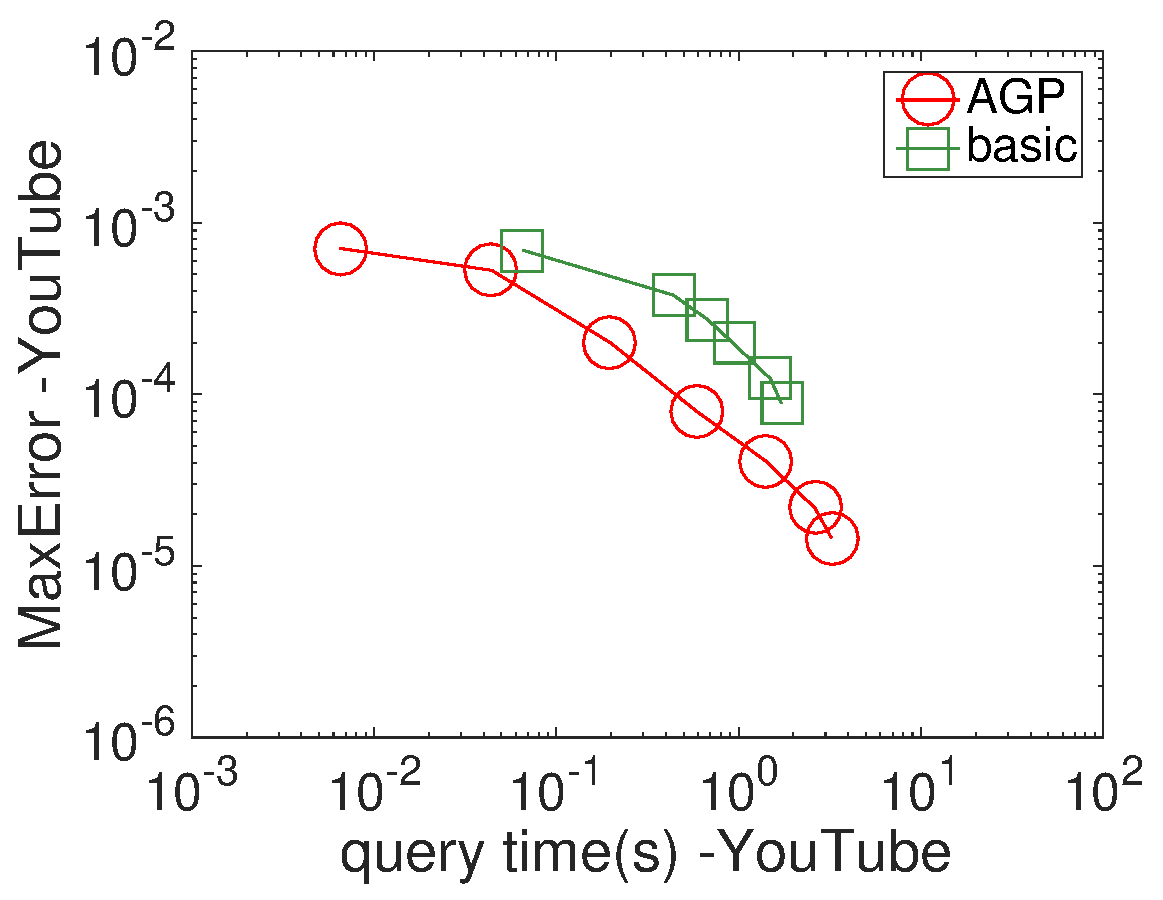
\includegraphics[height=34.5mm]{./Figs/Katz-maxerr-query-YT.eps} &
			\hspace{-4.4mm} 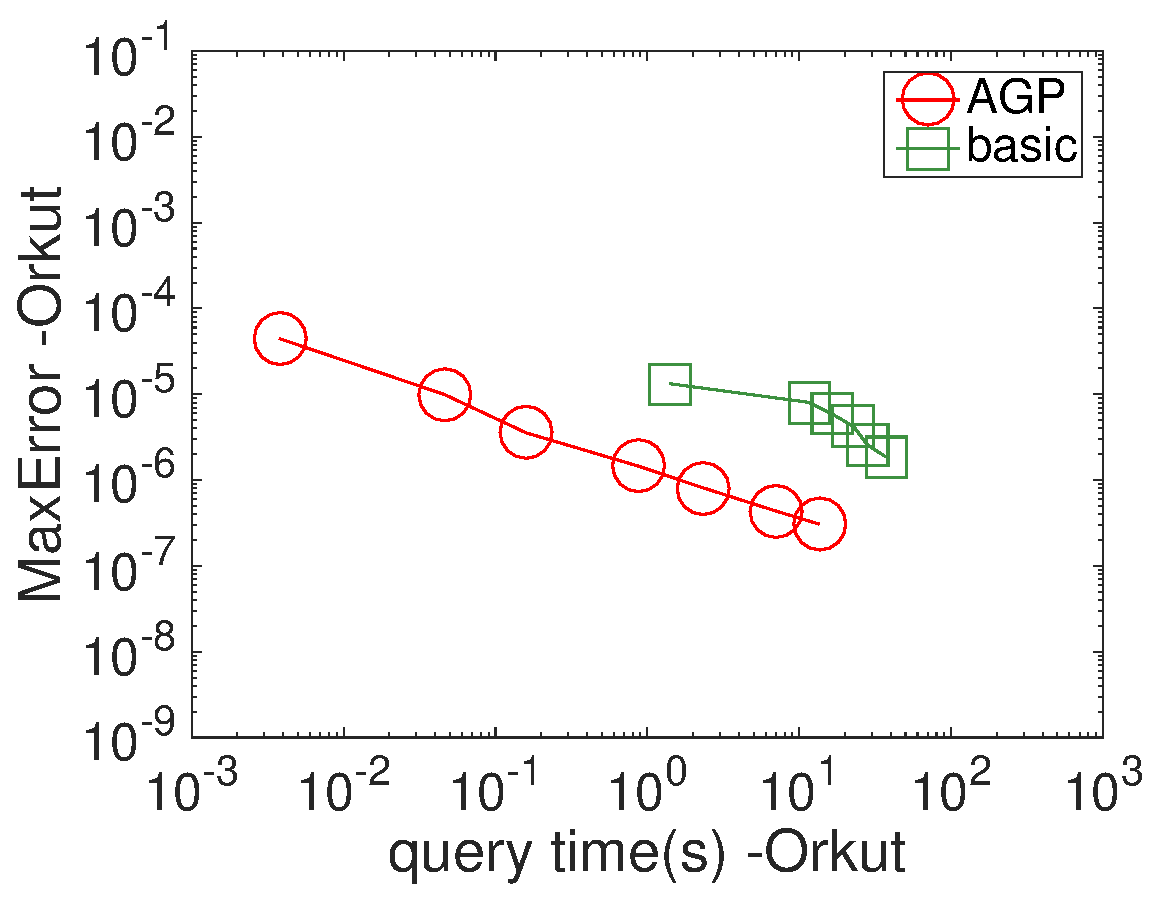
\includegraphics[height=34.5mm]{./Figs/Katz-maxerr-query-OL.eps} &
			\hspace{-4.4mm} 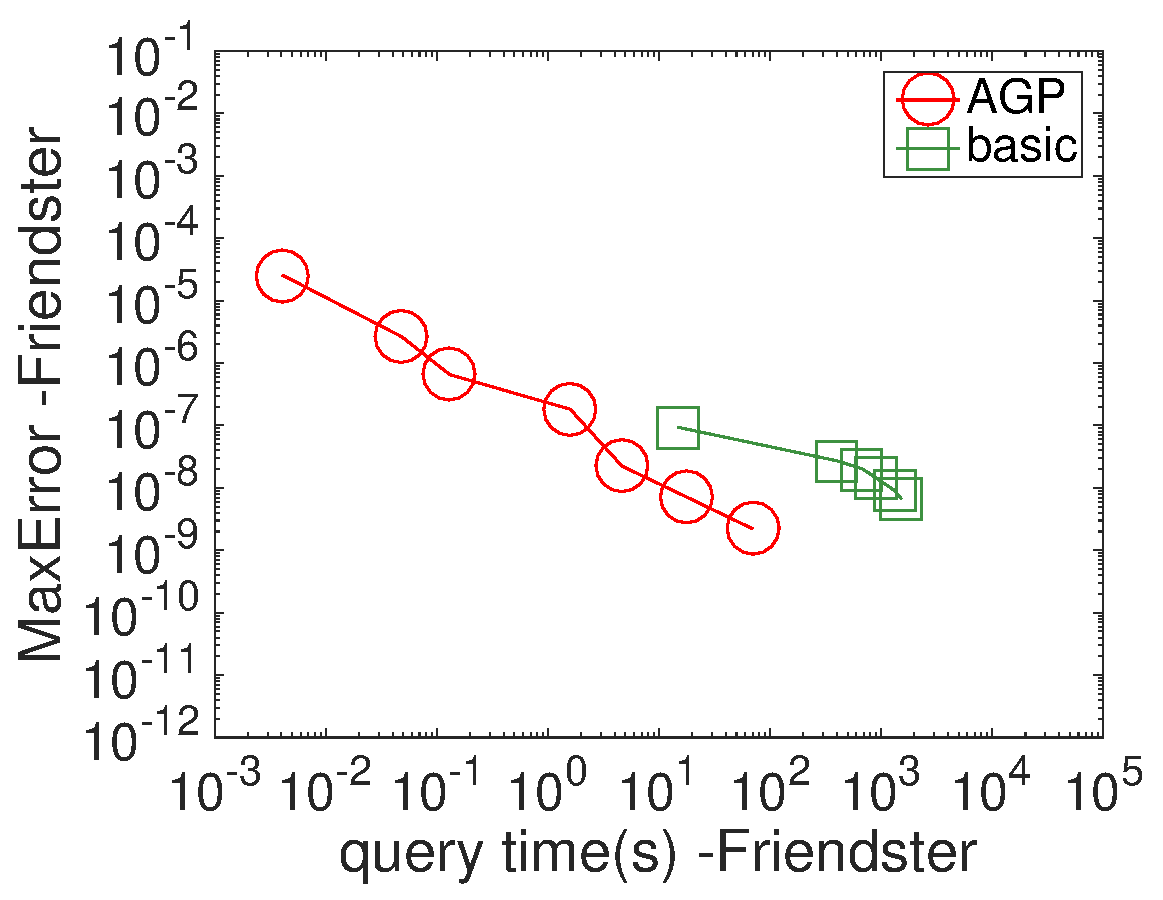
\includegraphics[height=34.5mm]{./Figs/Katz-maxerr-query-FR.eps} &
			\hspace{-4.4mm} 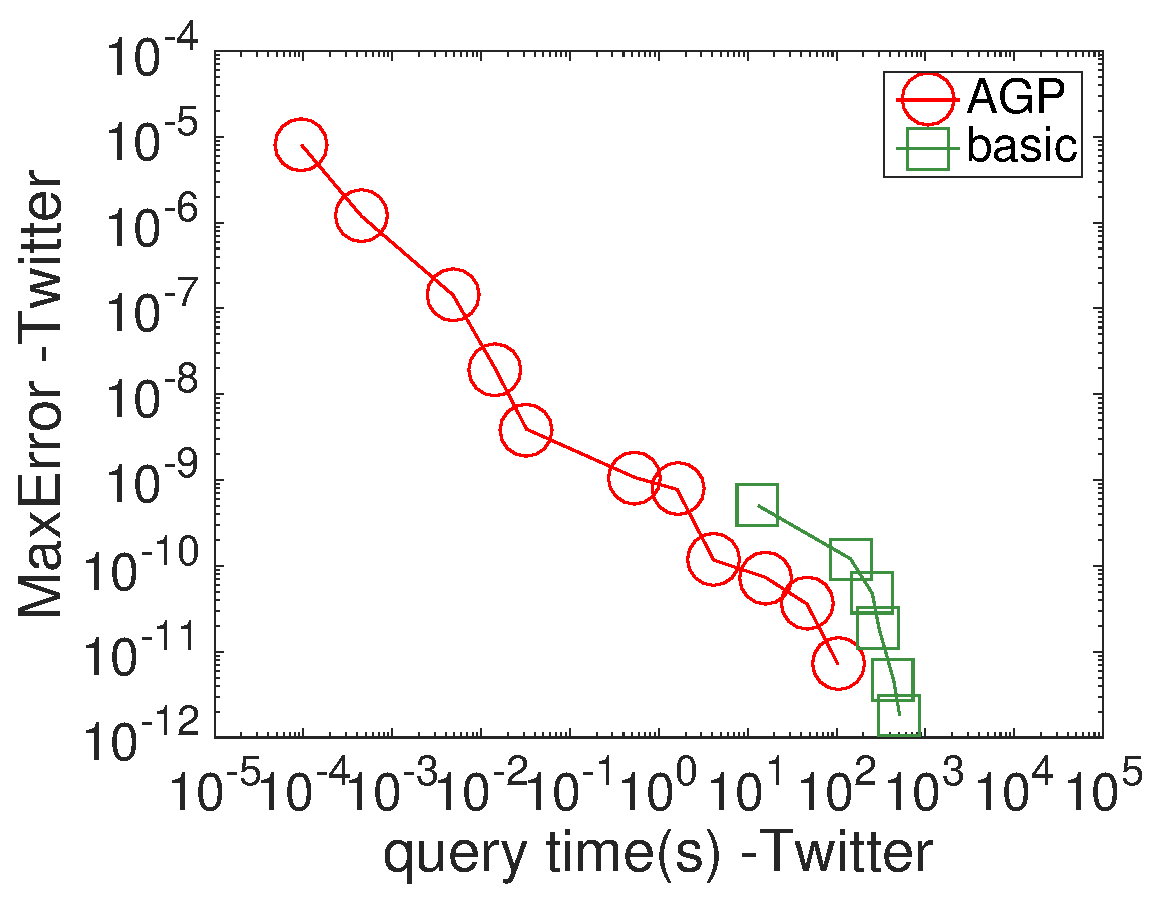
\includegraphics[height=34.5mm]{./Figs/Katz-maxerr-query-TW.eps} 
		\end{tabular}
		\vspace{-5mm}
		\caption{Tradeoffs between {\em MaxError} and query time of Katz.}
		\label{fig:Katz-MaxError-query}
		\vspace{-2mm}
	\end{small}
\end{figure*}


\begin{figure*}[t]
	\begin{small}
		\centering
		\vspace{-2mm}
		%    \begin{footnotesize}
		\begin{tabular}{cccc}
			%\multicolumn{4}{c}{\hspace{-4mm} \includegraphics[height=5mm]{./Figs/legend_large.eps}} \vspace{-1mm} \\
			\hspace{-4mm} 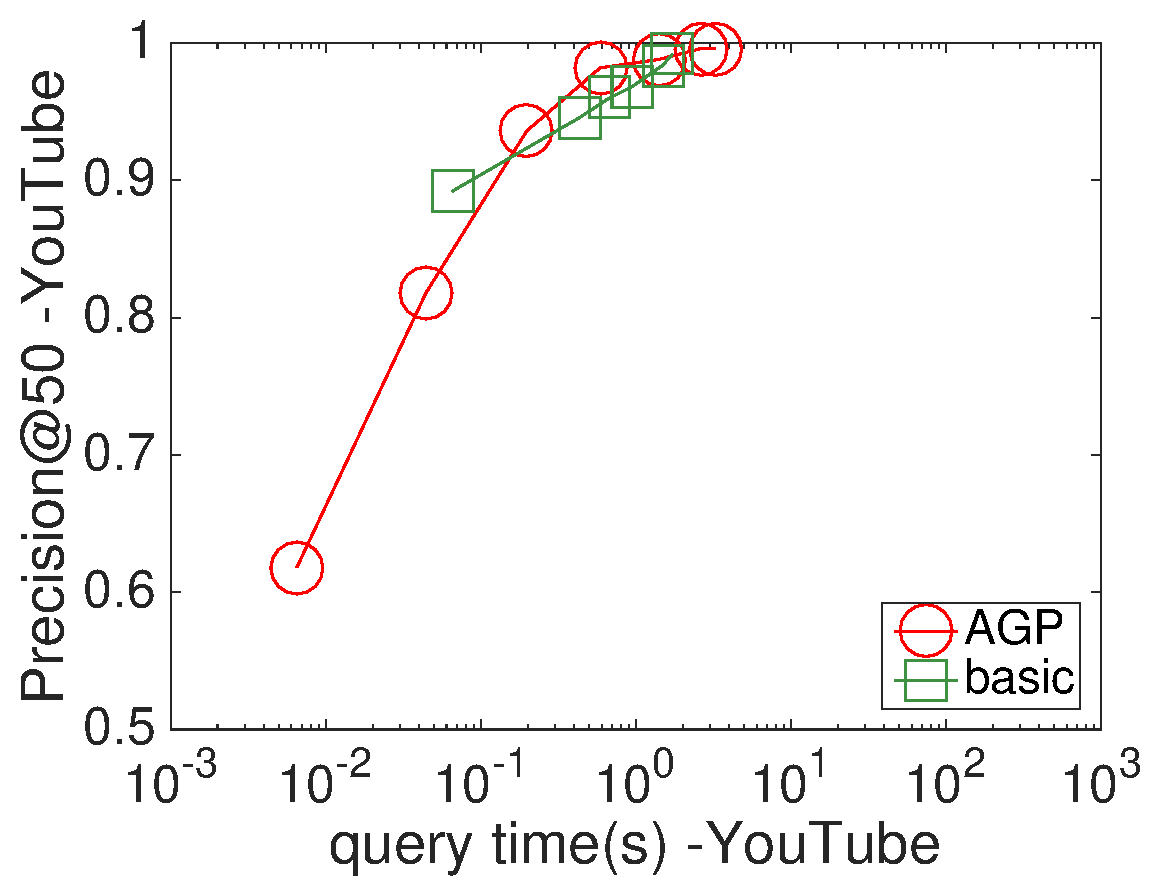
\includegraphics[height=33.8mm]{./Figs/Katz-precision-query-YT.eps} &
			\hspace{-4mm} 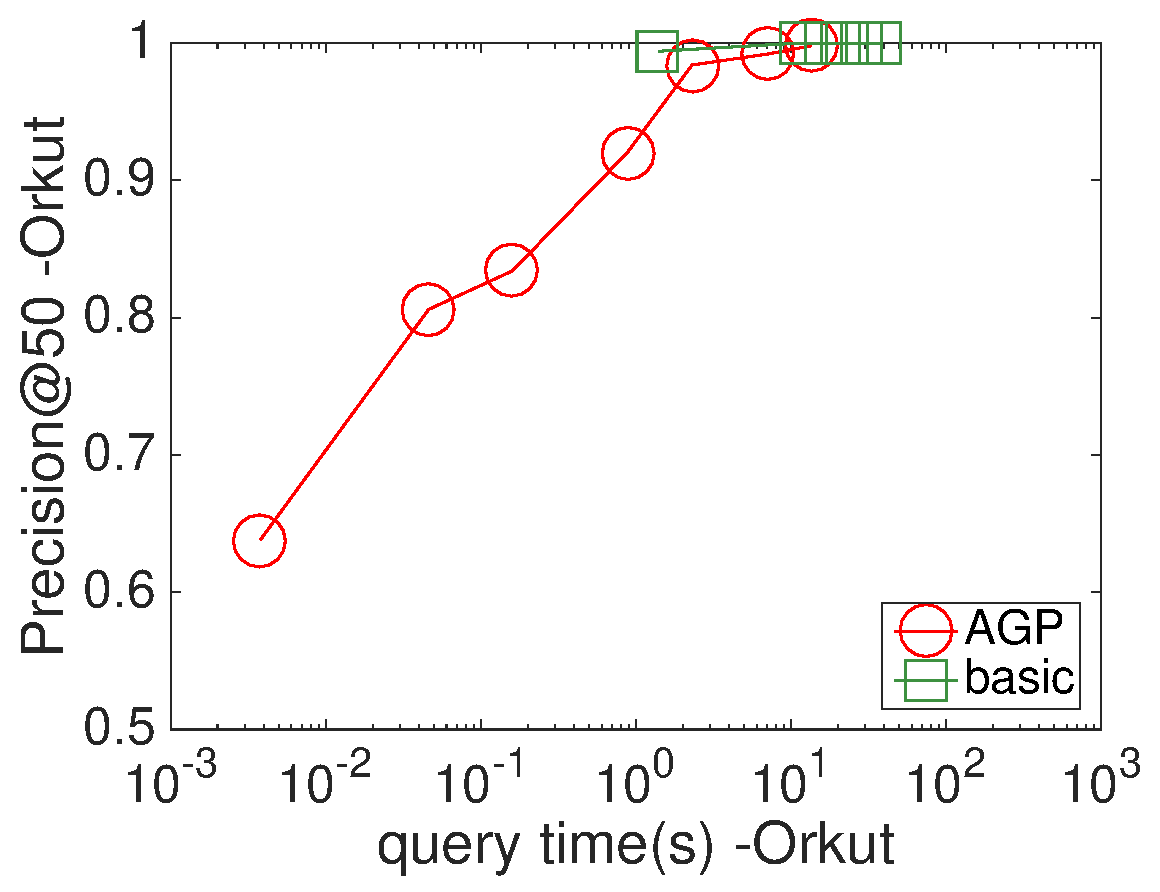
\includegraphics[height=33.8mm]{./Figs/Katz-precision-query-OL.eps} &
			\hspace{-4mm} 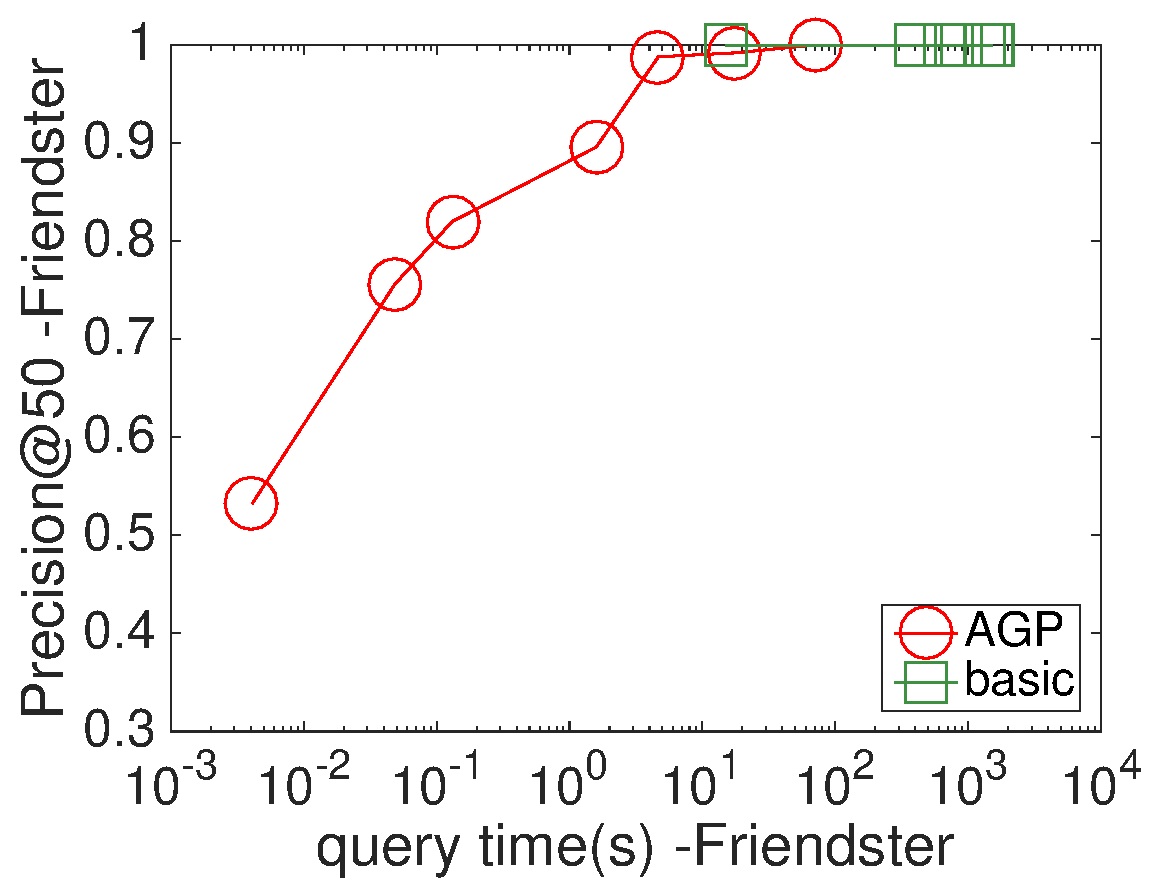
\includegraphics[height=33.8mm]{./Figs/Katz-precision-query-FR.eps} &
			\hspace{-4mm} 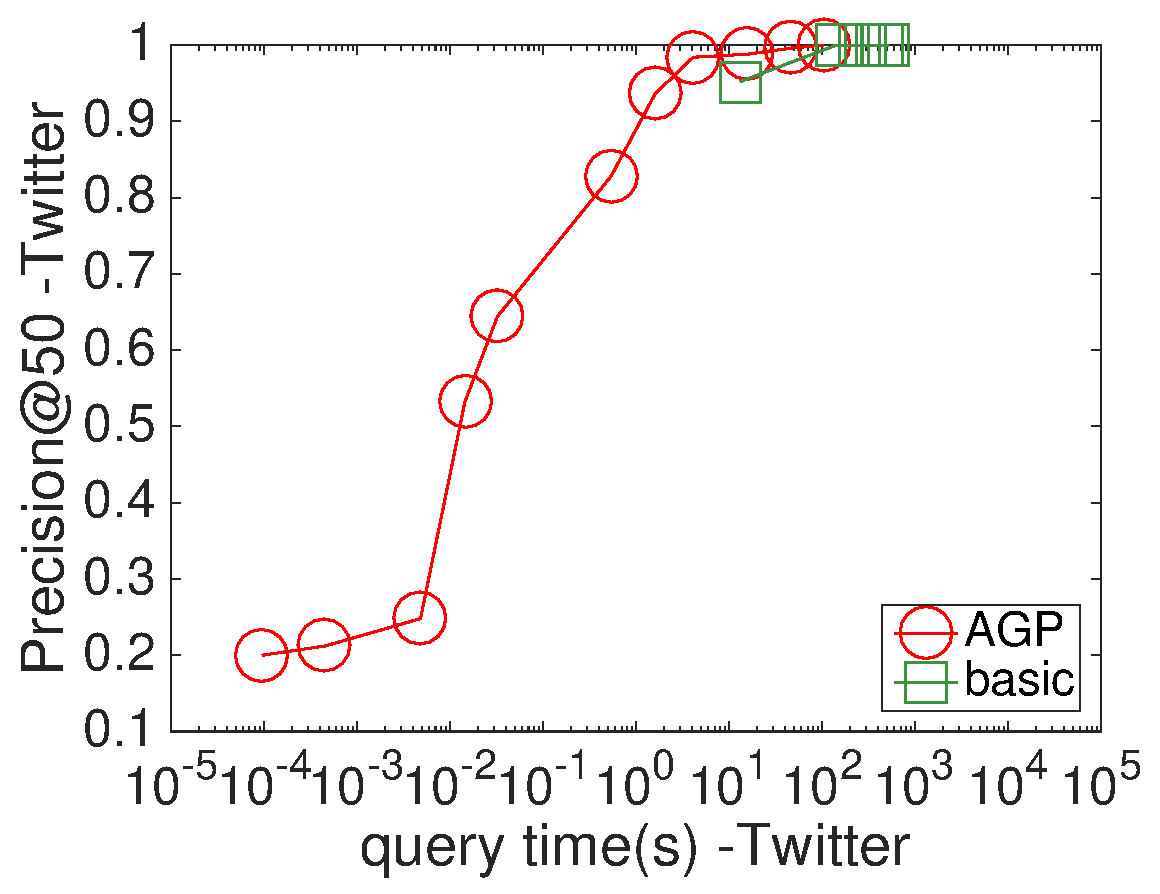
\includegraphics[height=33.8mm]{./Figs/Katz-precision-query-TW.eps} 
		\end{tabular}
		\vspace{-5mm}
		\caption{Tradeoffs between {\em Precision@50} and query time of Katz.}
		\label{fig:Katz-precision-query}
	    \vspace{-2mm}
	\end{small}
\end{figure*}

%\end{comment}



\section{Additional experimental results} \label{sec:appendix_old}
\subsection{Local clustering with HKPR}
%\header{\bf Comparison of overhead memory.} 
%Apart from the experiments shown in Section~\ref{subsec:clustering}, we further explore the memory cost of each method. 
Apart from using {\em MaxError} to measure the approximation quality, we further explore the trade-off curves between {\em Precision@k} and query time. 
%We use {\em Precision@k} as our metric to measure the approximation quality of each method. 
Let $V_k$ denote the set of $k$ nodes with highest normalized HKPR values, and $\hat{V}_k$ denote the estimated top-$k$ node set returned by an approximate method. {\em Normalized Precision@k} is defined as the percentage of nodes in $\hat{V}_k$ that coincides with the actual top-$k$ results $V_k$. {\em Precision@k} can evaluate the accuracy of the relative node order of each method. Similarly, we use the Basic Propagation Algorithm~\ref{alg:AGP-deter} with $L=50$ to obtain the ground truths of the normalized HKPR. %On directed graph, $d_v$ is substituted by the out-degree $d_{out}(v)$. 
Figure~\ref{fig:HKPR-precision-query} plots the trade-off curve between {\em Precision@50} and the query time for each method. We omit TEA and TEA+ on Twitter as they cannot handle directed graphs. We observe that AGP achieves the highest precision among the five approximate algorithms on all four datasets under the same query time. 
%Figure~\ref{fig:HKPR-conductance-mem} plots the trade-off lines between conductance and overhead memory. We exclude the space cost by the input graph in overhead memory. We can observe that the memory cost of AGP is relative small among these competitors. On {\em Friendster}, AGP can save $10\times$ space than TEA and TEA+. Moreover, we find that the overhead memory of each method is merely unchanged, which means the error bound only has a limited influence on memory cost. 

Besides, we also conduct experiments to present the influence of heat kernel parameter $t$ on the experimental performances. Figure~\ref{fig:conductance-query-OL} plots the conductance and query time trade-offs on {\em Orkut}, with $t$ varying in $\{5,10,20,40\}$. Recall that $t$ is the average length of the heat kernel random walk. Hence, the query time of each method increases as $t$ varying from 5 to 40.  We observe that AGP consistently achieves the lowest conductance with the same amount of query time. Furthermore, as $t$ increases from $5$ to $40$, AGP's query time only increases by $7\times$, while TEA and TEA+ increase by $10\times-100\times$, which demonstrates the scalability of AGP. 

%Besides, we also present Figure~\ref{fig:HKPR-conductance-query-YT} to show the conductance trade-offs with varying heat kernel parameter $t$ on {\em Youtube}. Observe that AGP can consistently outperform other competitors with varying $t$, which reflects the stability of AGP with different parameters and datasets.


%\vspace{-1mm}
\subsection{Evaluation of Katz index}

\begin{figure*}[t]
%	\begin{small}
		\centering
		\vspace{-1mm}
		%    \begin{footnotesize}
		\begin{tabular}{cccc}
			%\multicolumn{4}{c}{\hspace{-4mm} \includegraphics[height=5mm]{./Figs/legend_large.eps}} \vspace{-1mm} \\
			%\hspace{-3mm} 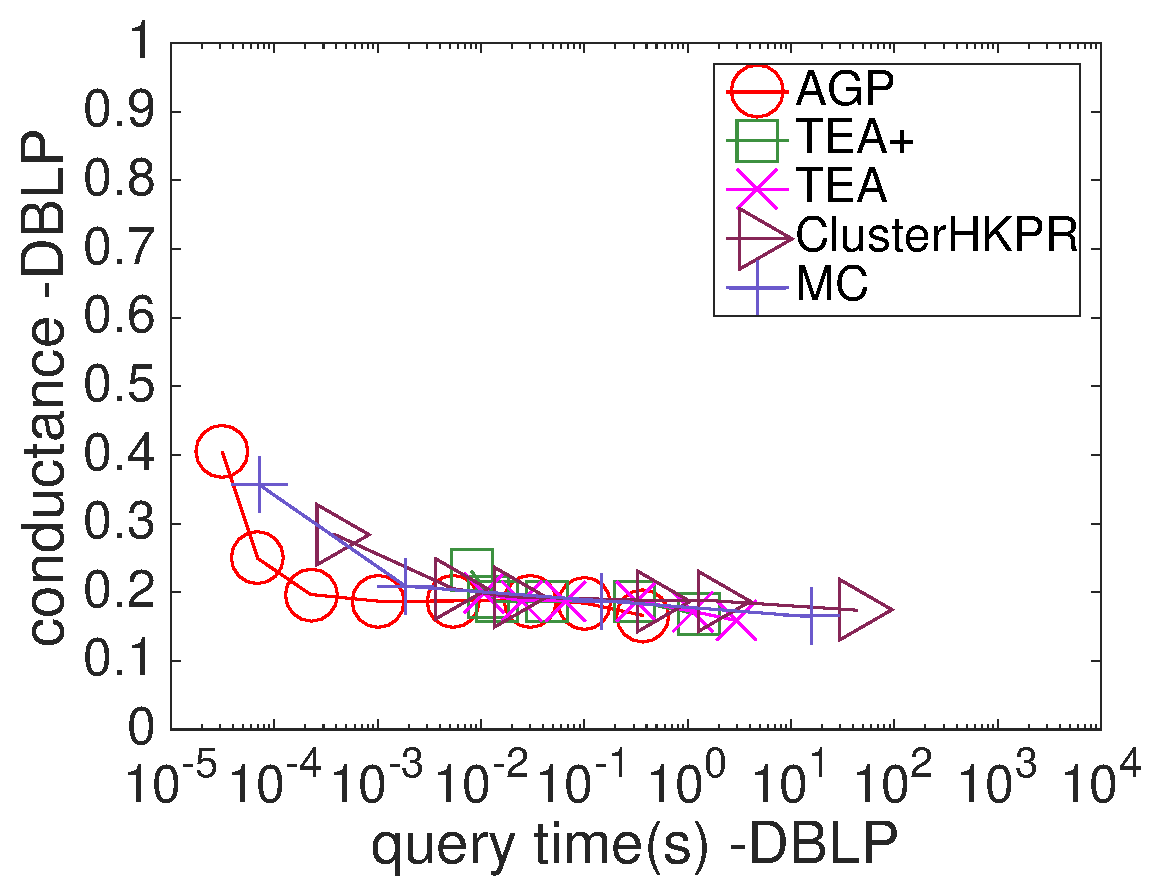
\includegraphics[height=25mm]{./Figs/HKPR-conductance-query-DB.eps} &
			\hspace{-4mm} 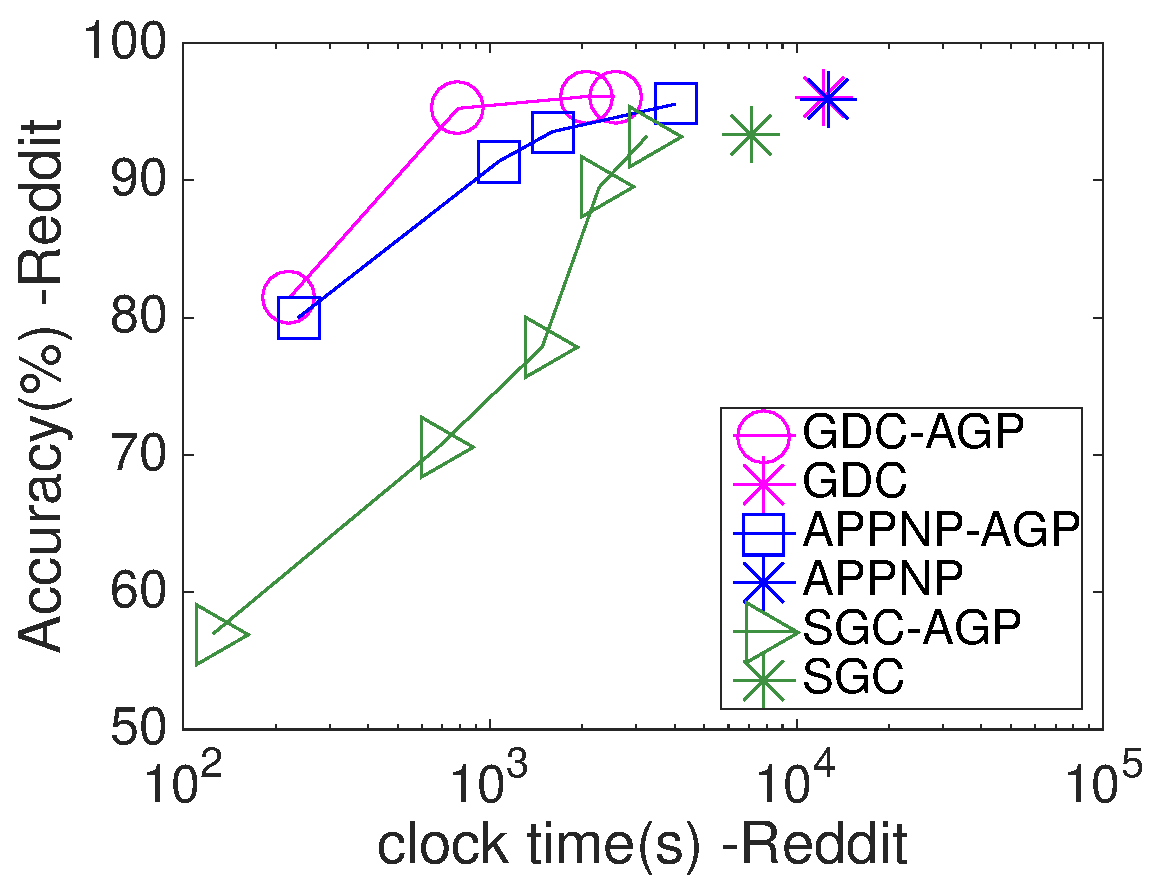
\includegraphics[height=34mm]{./Figs/GNN-accuracy-clock-Reddit.eps} &
			\hspace{-2mm} 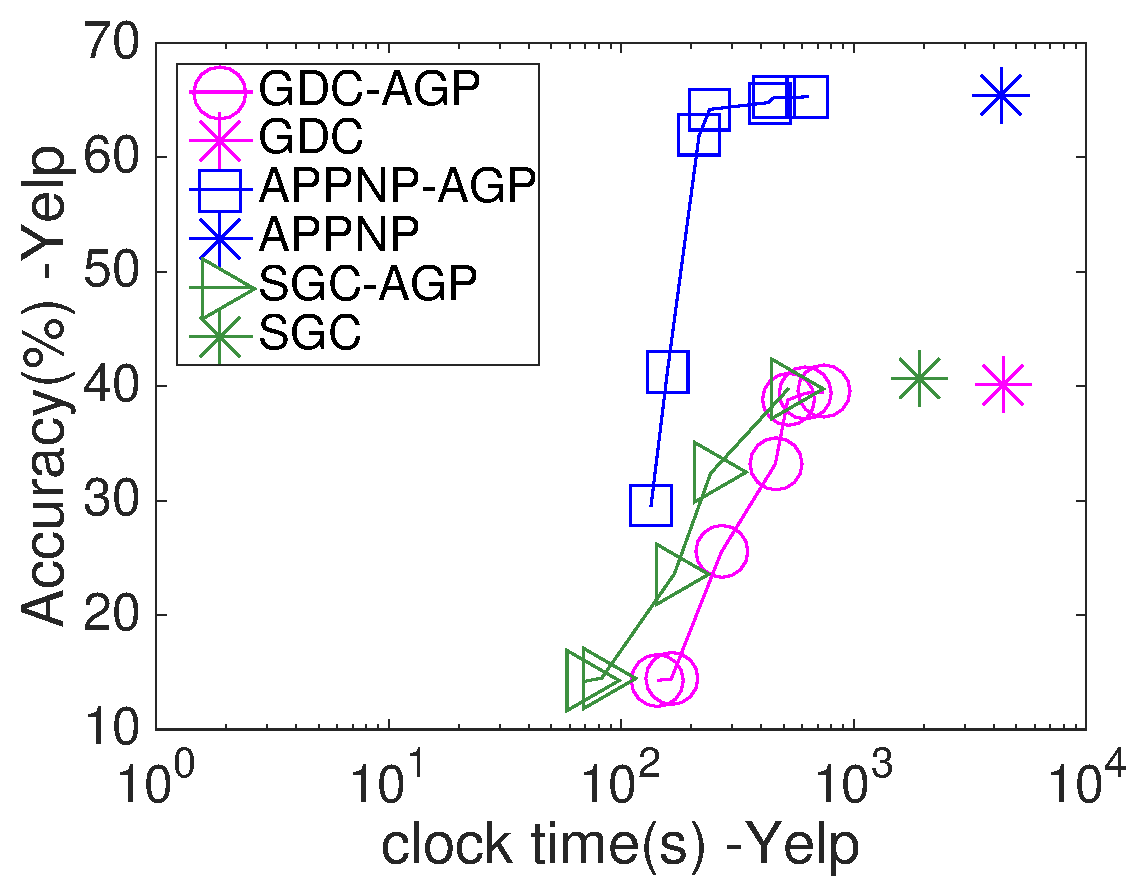
\includegraphics[height=34mm]{./Figs/GNN-accuracy-clock-Yelp.eps} &
			\hspace{-4mm} 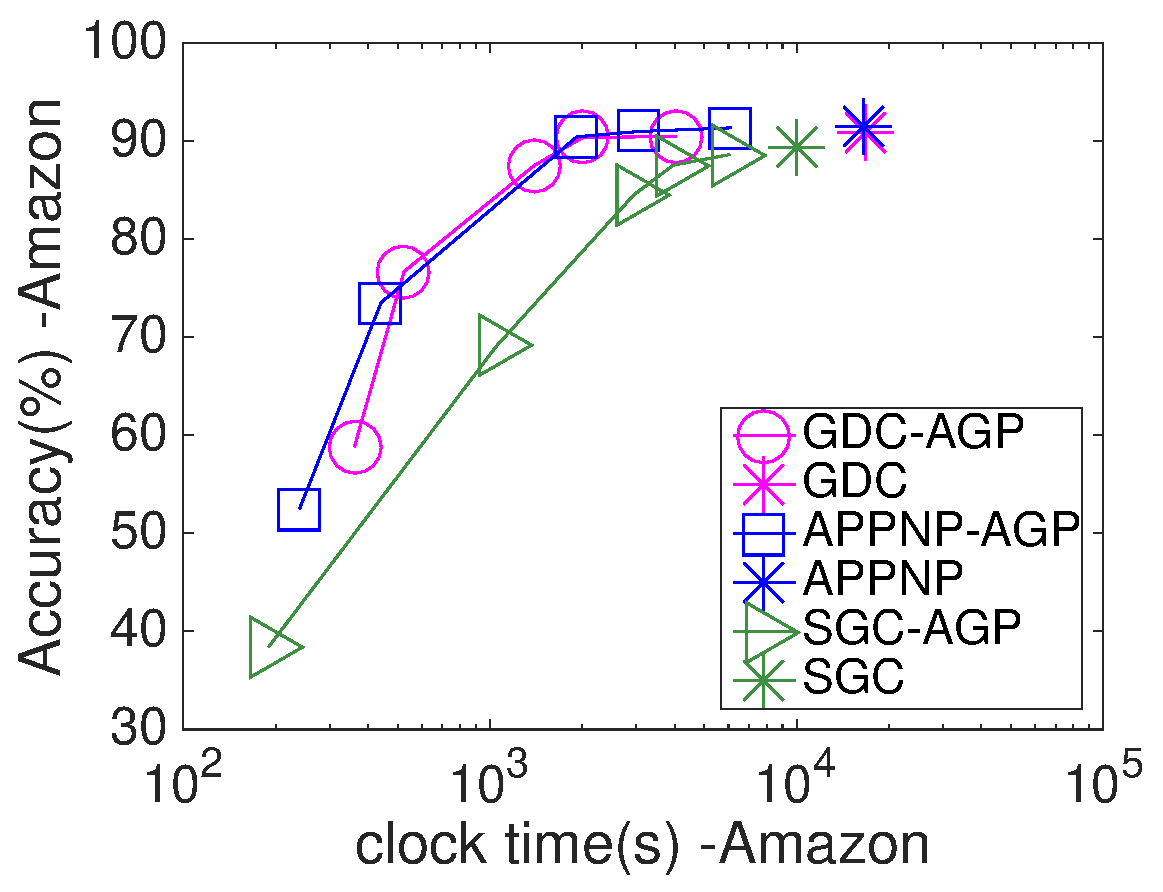
\includegraphics[height=34mm]{./Figs/GNN-accuracy-clock-Amazon.eps} &
			\hspace{-4mm} 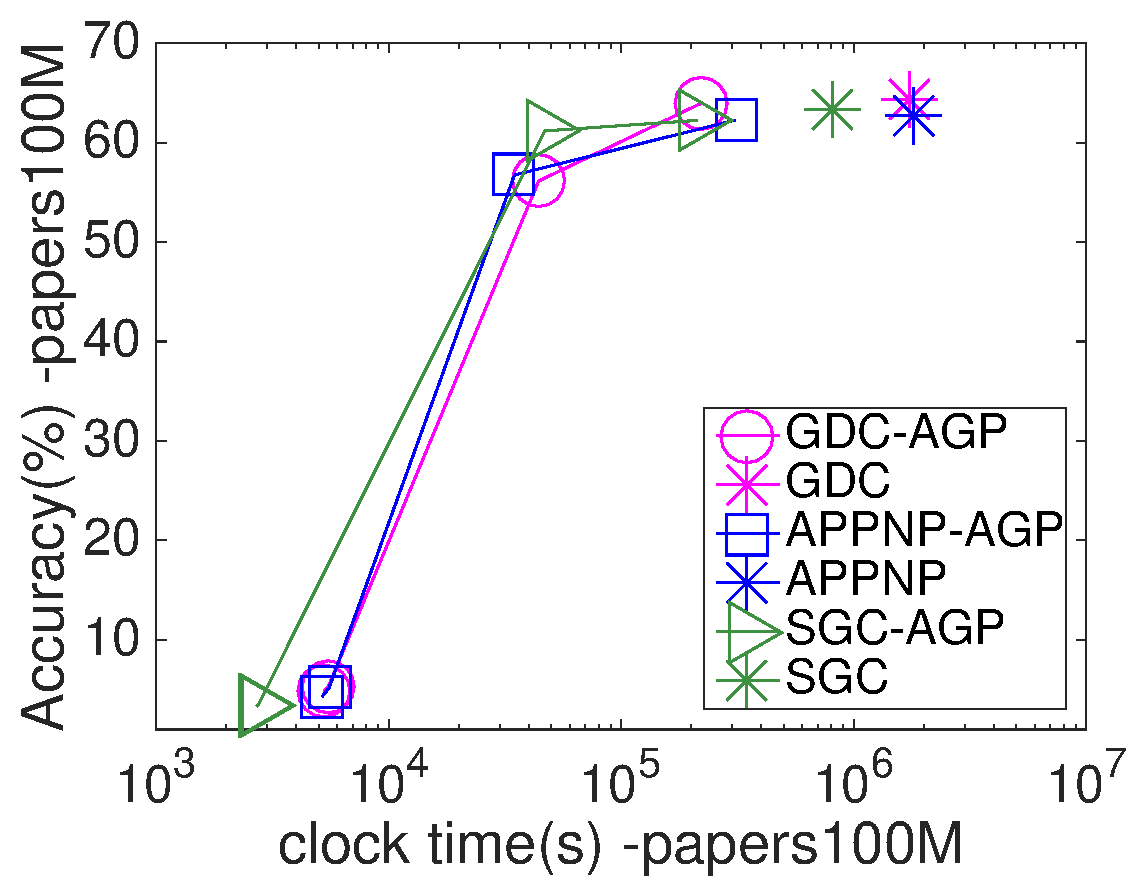
\includegraphics[height=34mm]{./Figs/GNN-accuracy-clock-papers100M.eps} 
		\end{tabular}
		\vspace{-5mm}
		\caption{Tradeoffs between {\em Accuracy(\%)} and clock time in node classification.}
		\label{fig:GNN-accuracy-clock-time}
		\vspace{-1mm}
%	\end{small}
\end{figure*}





%\begin{comment}
%\header{\bf Katz index.}
We also evaluate the performance of AGP to compute the Katz index. Recall that Katz index numerates the paths of all lengths between a pair of nodes, which can be expressed as that $\vec{\pi}=\sum_{i=0}^\infty \beta^i \cdot \mathbf{A}^{i} \cdot \vec{e}_s$. 
%\begin{align}\nonumber
%	\vec{\pi}=\sum_{i=0}^\infty \beta^i \cdot \mathbf{A}^{i} \cdot \vec{e}_s. 
%	%\vspace{-2mm}
%\end{align}
%In our experiments, $\beta$ is set as $\frac{0.85}{\lambda_1}$ to guarantee convergence, where $\lambda_1$ denotes the largest eigenvalue of the adjacent matrix $\bm{A}$. We compare the performance of AGP with the basic propagation algorithm given in Algorithm~\ref{alg:AGP-deter} (denoted as basic in Figure~\ref{fig:Katz-MaxError-query},~\ref{fig:Katz-precision-query}). We treat the results computed by the basic propagation algorithm with $L=50$ as the ground truths. Varying $\delta$ from $0.01$ to $10^{8}$, Figure~\ref{fig:Katz-MaxError-query} shows the trade-offs between {\em MaxError} and query time. Here we define $MaxError =\max_{v \in V}\left|\vec{\pi}(v)-\vec{\epi}(v)\right|$. We issue 50 query nodes and return the average {\em MaxError} of all query nodes same as before. We can observe that AGP costs less time than basic propagation algorithm to achieve the same error. Especially when $\delta$ is large, such as $MaxError=10^{-5}$ on the dataset {\em Orkut}, AGP has a $10\times-100\times$ speed up than the basic propagation algorithm. Figure~\ref{fig:Katz-precision-query} plots the trade-off lines between {\em Precision@50} and query time. Note that the basic propagation algorithm can always achieve precision 1 even with large {\em MaxError}. This is because the propagation results derived by the basic propagation algorithm are always smaller than the ground truths. The biased results may present large error and high precision simultaneously by maintaining the relative order of top-k nodes. While AGP is not a biased method, the precision will increase with the decreasing of {\em MaxError}. 
In our experiments, $\beta$ is set as $\frac{0.85}{\lambda_1}$ to guarantee convergence, where $\lambda_1$ denotes the largest eigenvalue of the adjacent matrix $\bm{A}$. We compare the performance of AGP with the basic propagation algorithm given in Algorithm~\ref{alg:AGP-deter} (denoted as basic in Figure~\ref{fig:Katz-MaxError-query}, ~\ref{fig:Katz-precision-query}). We treat the results computed by the basic propagation algorithm with $L=50$ as the ground truths. Varying $\delta$ from $0.01$ to $10^{8}$, Figure~\ref{fig:Katz-MaxError-query} shows the trade-offs between {\em MaxError} and query time. Here we define $MaxError =\max_{v \in V}\left|\vec{\pi}(v)-\vec{\epi}(v)\right|$. We issue 50 query nodes and return the average {\em MaxError} of all query nodes same as before. We can observe that AGP costs less time than basic propagation algorithm to achieve the same error. Especially when $\delta$ is large, such as $MaxError=10^{-5}$ on the dataset {\em Orkut}, AGP has a $10\times-100\times$ speed up than the basic propagation algorithm. Figure~\ref{fig:Katz-precision-query} plots the trade-off lines between {\em Precision@50} and query time. The definition of {\em Precision@k} is the same as Figure~\ref{fig:HKPR-precision-query}, which equals the percentage of nodes in the estimated top-k set that coincides with the real top-k nodes. 
Note that the basic propagation algorithm can always achieve precision 1 even with large {\em MaxError}. This is because the propagation results derived by the basic propagation algorithm are always smaller than the ground truths. The biased results may present large error and high precision simultaneously by maintaining the relative order of top-k nodes. While AGP is not a biased method, the precision will increase with the decreasing of {\em MaxError}. 

%\end{comment}


%large error, but the relative order of top-k nodes may be accurate. 
%This concurs with our analysis that the basic propagation algorithm can return high accuracy results with expensive time cost. 




\vspace{-1mm}
\subsection{Node classification with GNN}
\header{\bf Comparison of clock time.}
To eliminate the effect of parallelism, we plot the trade-offs between clock time and classification accuracy in Figure~\ref{fig:GNN-accuracy-clock-time}. We can observe that AGP still achieves a $10\times$ speedup on each dataset, which concurs with the analysis for propagation time. Besides, note that every method presents a nearly $30\times$ speedup after parallelism, which reflects the effectiveness of parallelism. 








%\begin{figure}[h]
%	\begin{small}
%		\centering
%		\vspace{-4mm}
%		%    \begin{footnotesize}
%		\begin{tabular}{cccc}
%			%\multicolumn{4}{c}{\hspace{-4mm} %\includegraphics[height=5mm]{./Figs/legend_large.eps}} \vspace{-1mm} \\
%			%\hspace{-3mm} %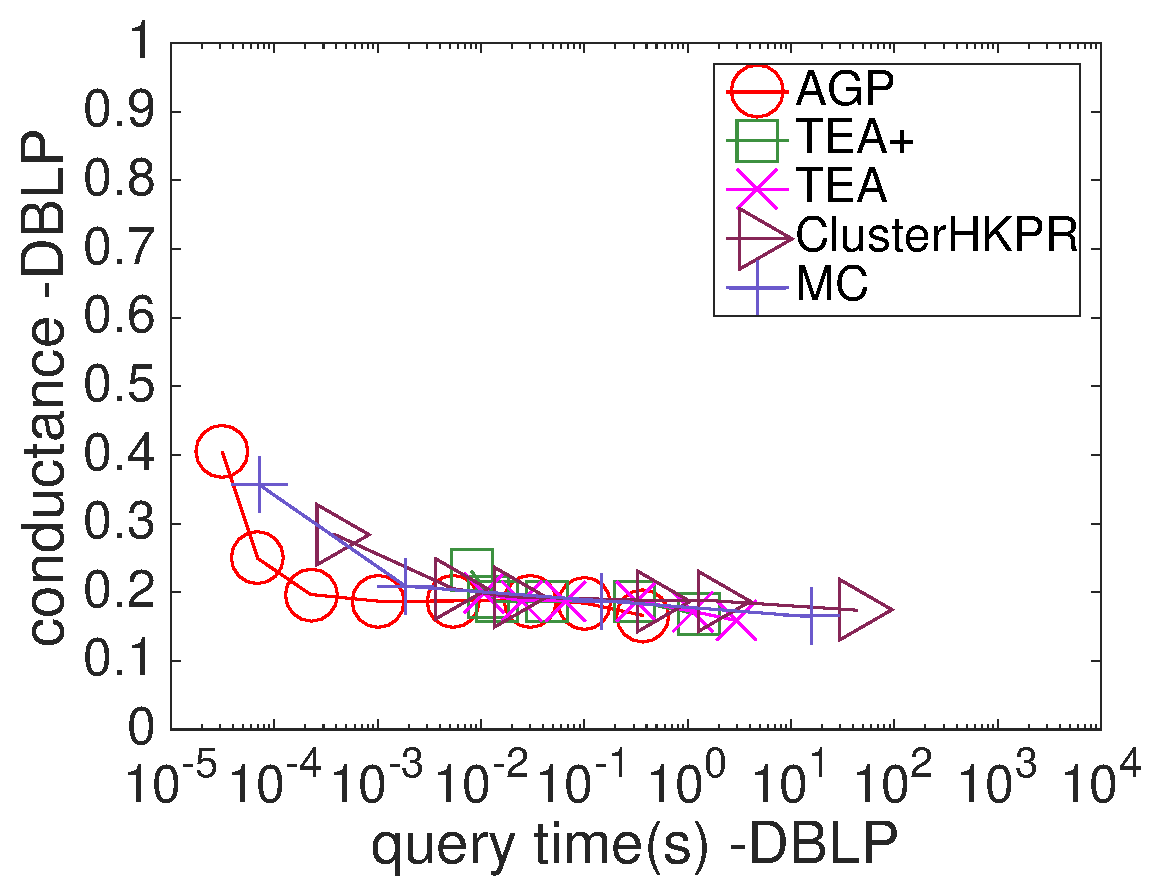
\includegraphics[height=25mm]{./Figs/HKPR-conductance-query-DB.eps} &
%			\hspace{-4mm} \includegraphics[height=45mm]{./Figs/bbb.eps} &
%		\end{tabular}
%		\vspace{-3mm}
%		\caption{Propagation time v.s. training time}
%		\label{fig:GNN-propagation-training}
%		\vspace{-4mm}
%	\end{small}
%\end{figure}

\begin{figure}[t]
	\begin{small}
		\centering
		%\vspace{-2mm}
		%    \begin{footnotesize}
		\begin{tabular}{cccc}
			%\multicolumn{4}{c}{\hspace{-4mm} \includegraphics[height=5mm]{./Figs/legend_large.eps}} \vspace{-1mm} \\
			%\hspace{-3mm} 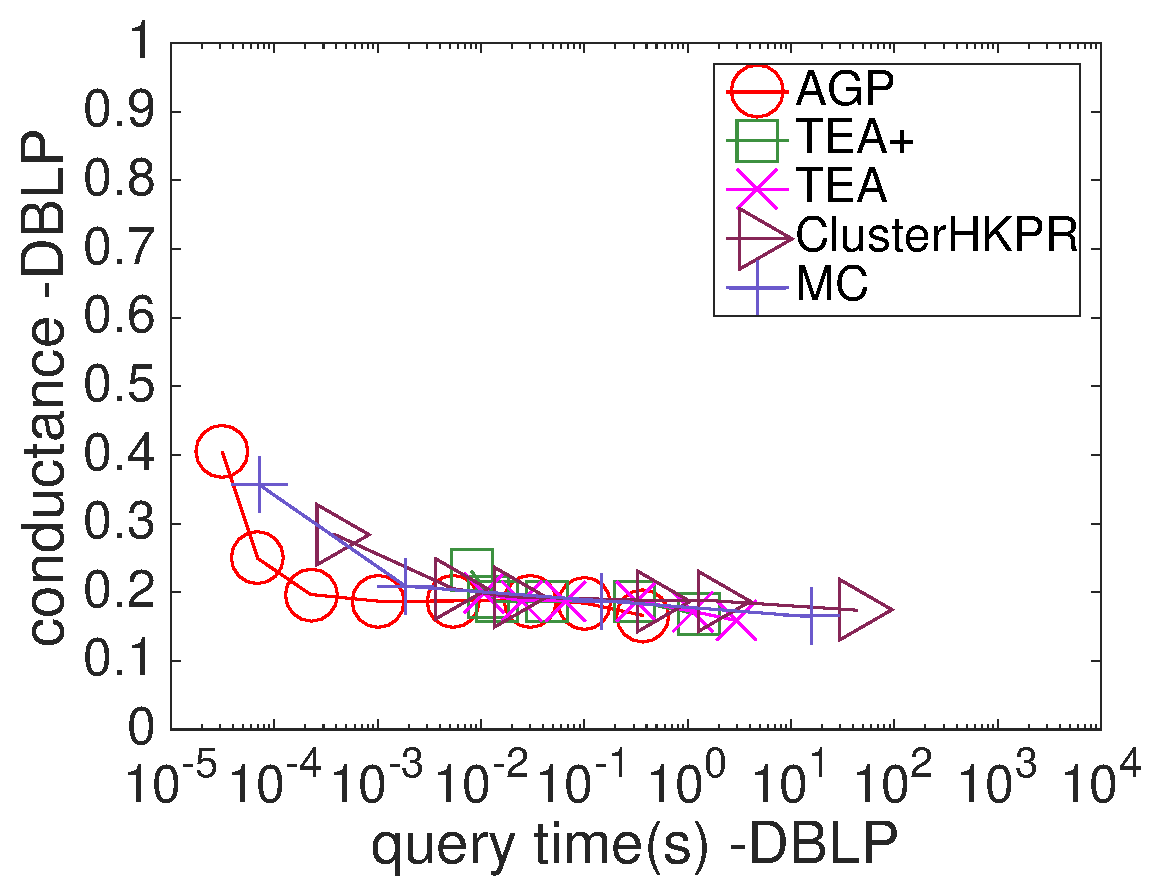
\includegraphics[height=25mm]{./Figs/HKPR-conductance-query-DB.eps} &
			%\hspace{-4mm} %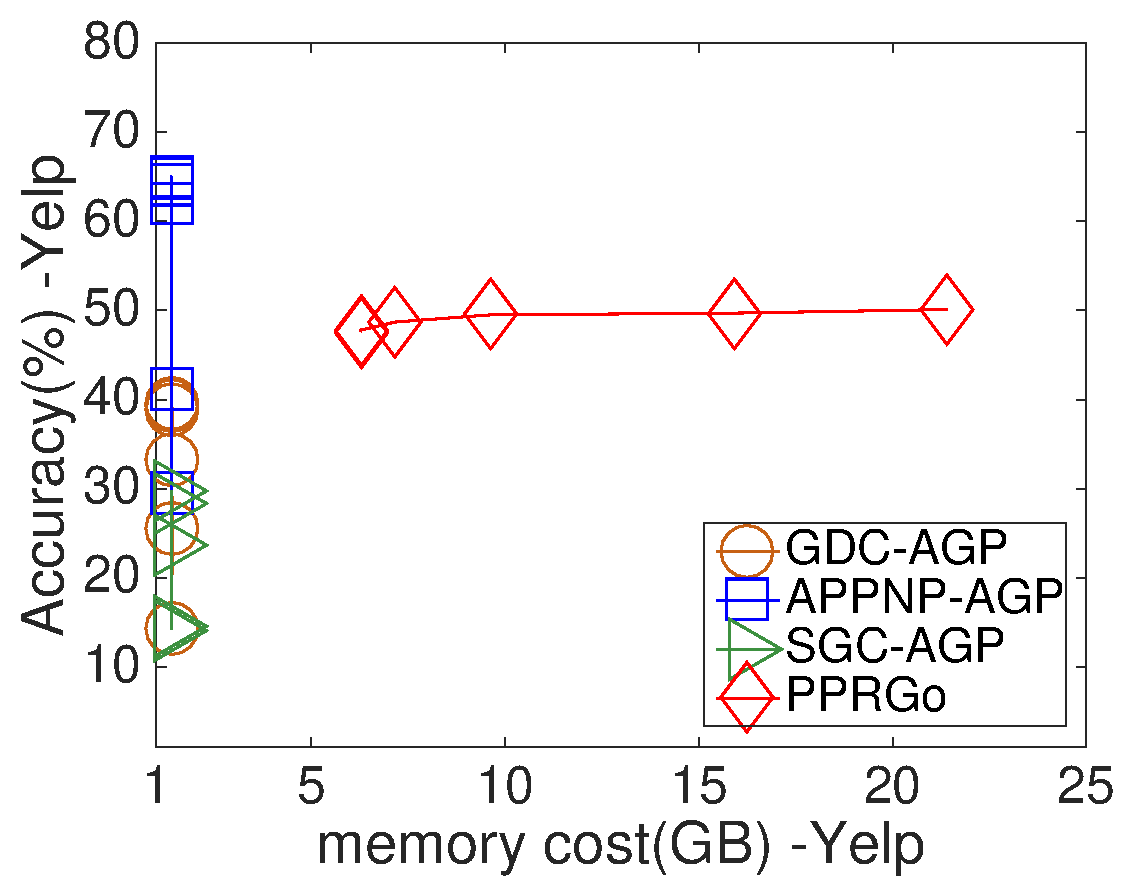
\includegraphics[height=34mm]{./Figs/GNN-accuracy-memory-Yelp.eps} &
			\hspace{-3mm} 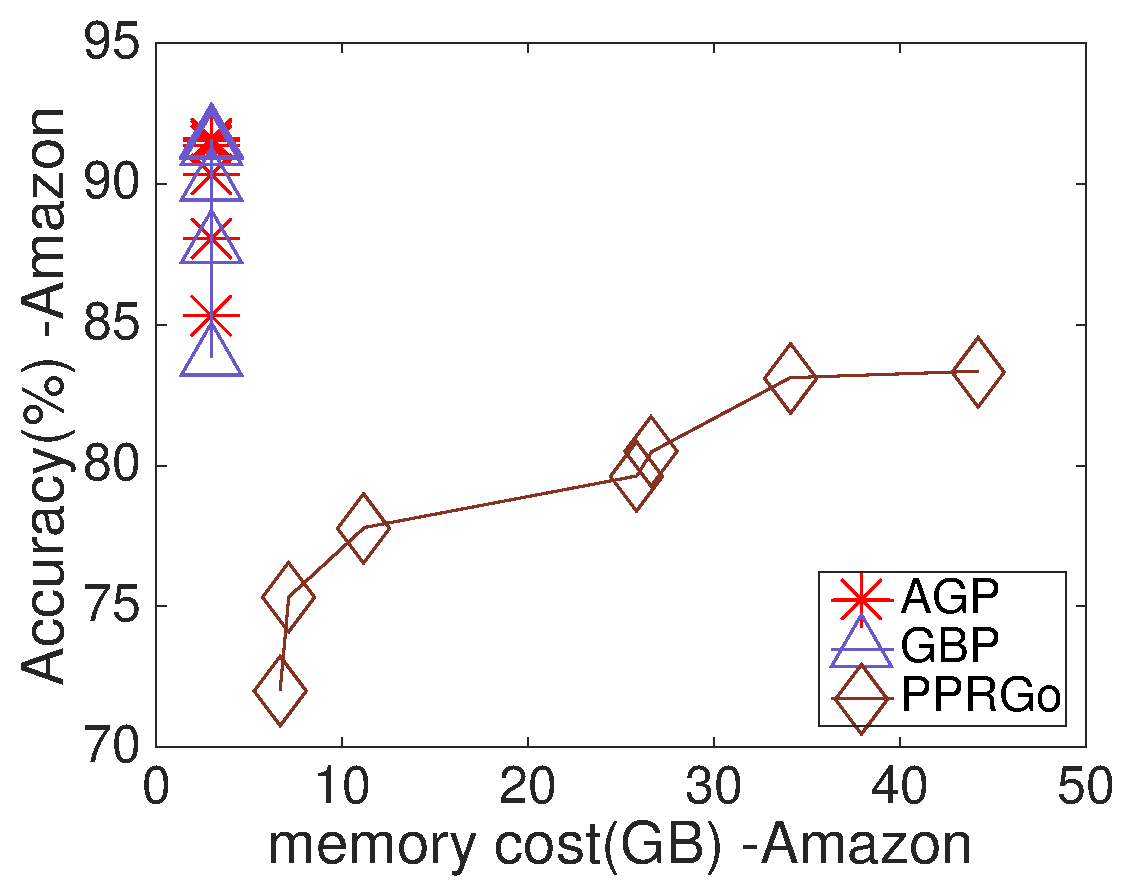
\includegraphics[height=32mm]{./Figs/GNN-accuracy-memory-Amazon.eps} &
			%\hspace{-4mm} %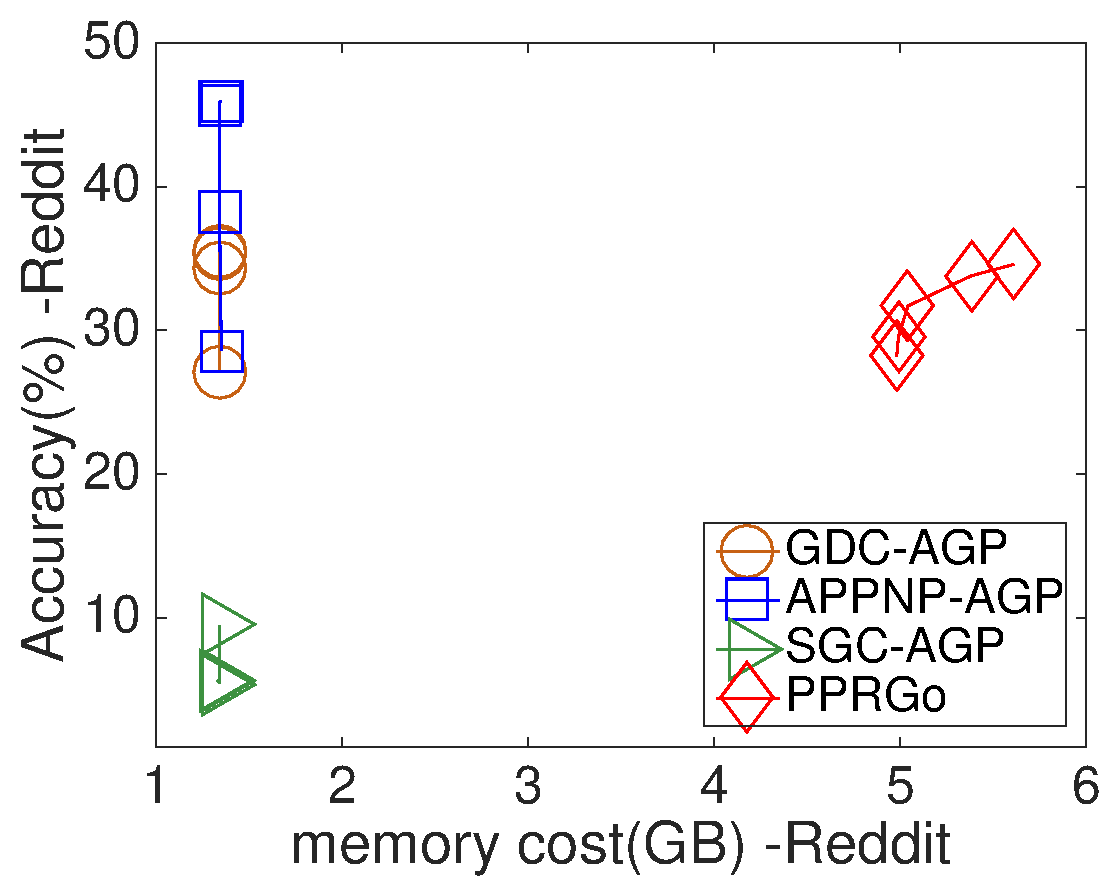
\includegraphics[height=34mm]{./Figs/GNN-accuracy-memory-Reddit.eps} &
			\hspace{-1mm} 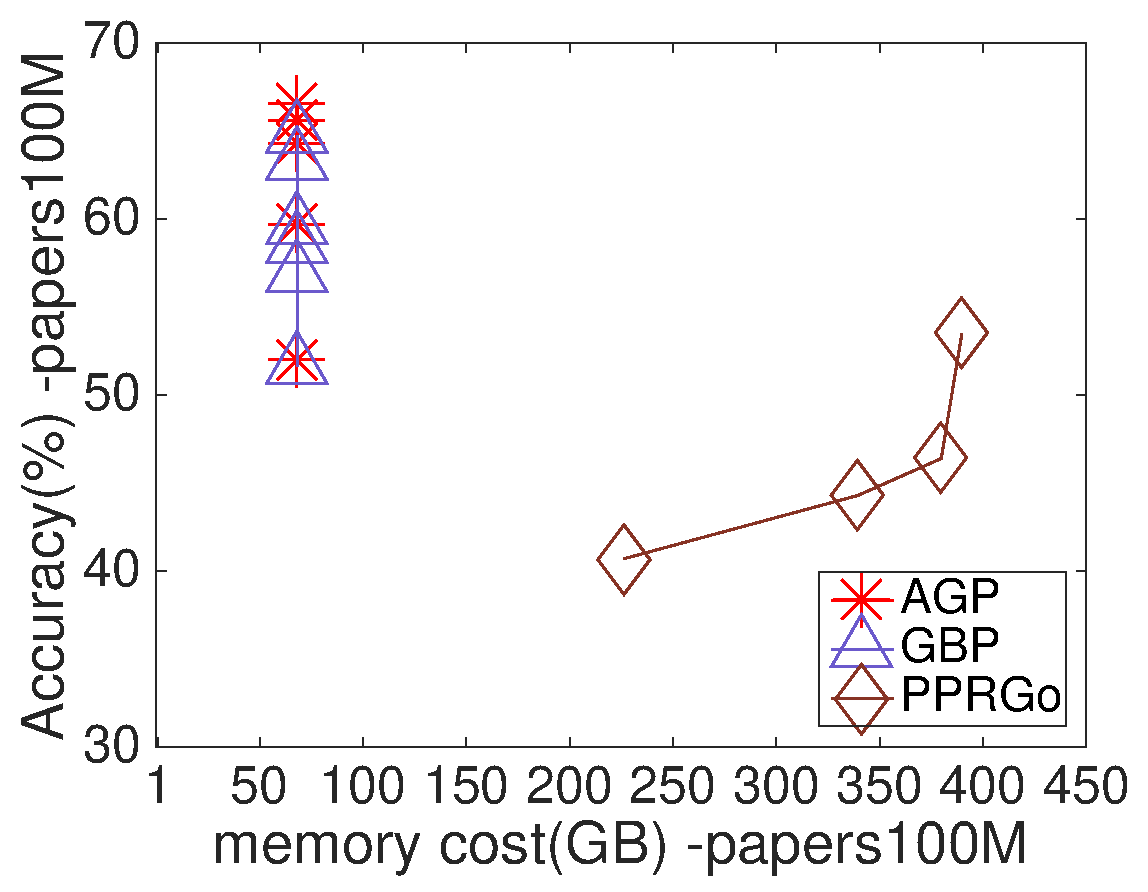
\includegraphics[height=32mm]{./Figs/GNN-accuracy-memory-papers100M.eps} 
		\end{tabular}
		\vspace{-5mm}
		\caption{Tradeoffs between {\em Accuracy(\%)} and memory cost in node classification.}
		\label{fig:GNN-accuracy-memory}
		\vspace{-4mm}
	\end{small}
\end{figure}



\header{\bf Comparison of preprocessing time and training time. }
Table~\ref{tbl:propagation-training} shows the comparison between the training time and preprocessing time on Papers100M. Due to the large batch size (10000), the training process is generally significantly faster than the feature propagation process. Hence, we recognize feature propagation as the bottleneck for scaling GNN models on large graphs, motivating our study on approximate graph propagation.





\header{\bf Comparison of memory cost. }
Figure~\ref{fig:GNN-accuracy-memory} shows the memory overhead of AGP, GBP, and PPRGo. Recall that the AGP Algorithm~\ref{alg:AGP-RQ} only maintains two $n$ dimension vectors: the residue vector $\vec{r}$ and the reserve vector $\vec{q}$. Consequently, AGP only takes a fixed memory, which can be ignored compared to the graph's size and the feature matrix. Such property is ideal for scaling GNN models on massive graphs. %On the other hand, PPRGo requires a large memory size to store the intermediate local push results from each training node.


\begin{table}[h]
	%\vspace{-2mm}
	\centering
	\tblcapup
	\caption{preprocessing and training time}
	\vspace{-4mm}
	\tblcapdown
	\begin{small}
		\begin{tabular}{|c|r|r|r|r|} %p{0.8in}|}
		%\begin{tabular}{|p{1.8cm}|p{1.5cm}|p{1.3cm}|p{1.3cm}|p{0.7cm}|}
			\hline
			{\bf } & {\bf APPNP-AGP }\hspace{-1mm} & {\bf GDC-AGP} & {\bf SGC-AGP}& \makecell[c]{{\bf PPRGo}} \\ \hline
 \hspace{-1mm} \makecell[c]{preprocessing\\ time (s)} \hspace{-2mm} & 9253.85 \hspace{-1mm} &   6807.17& 1437.95 & 7639.72  \\ \hline
   \hspace{-1mm}training time (s)  \hspace{-2mm}  & 166.19  \hspace{-1mm}   & 175.62   & 120.07 & 140.67 \\
			\hline
		\end{tabular}
	\end{small}
	\label{tbl:propagation-training}
	%\tbldown
	%\vspace{-3mm}
\end{table}




\header{\bf Additional details in experimental setup.} 



%\begin{table}[h]
%	\vspace{-1mm}
	%\centering
	%\lefting
%	\tblcapup
%	\caption{Hyper-parameters of GBP.}
%	\vspace{-5mm}
%	\tblcapdown
%	\begin{small}
%		\begin{tabular}{|c|c|c|c|c|c|c|}\hline
%    \multirow{2}{*}{\bf Dataset} & {\bf Learning} & \multirow{2}{*}{\bf Dropout} & {\bf Hidden} & \multirow{2}{*}{\bf $r_{max}$} & \multirow{2}{*}{\bf $r$} & \multirow{2}{*}{\bf $\alpha$} \\ 
%    &{\bf rate}&& {\bf dimension} & & & \\ \hline
%    Amazon & 0.01 & 0.1 &1024& $10^{-7}$ & 0.2 & 0.2  \\ \hline
%    Papers100M & 0.0001 & 0.3 &2048& $10^{-8}$ & 0.5 & 0.2  \\ \hline
%	\end{tabular}
%	\end{small}
%	\label{tbl:para-GBP}
%	%\tbldown
%	\vspace{-2mm}
%\end{table}

%\begin{table}[h]
%	\vspace{-1mm}
	%\centering
	%\lefting
%	\tblcapup
%	\caption{Hyper-parameters of PPRGo.}
%	\vspace{-5mm}
%	\tblcapdown
%	\begin{small}
%		\begin{tabular}{|c|c|c|c|c|c|c|}\hline
%    \multirow{2}{*}{\bf Dataset} & {\bf Learning} & \multirow{2}{*}{\bf Dropout} & {\bf Hidden} & \multirow{2}{*}{\bf $k$} & \multirow{2}{*}{\bf $L$} & \multirow{2}{*}{\bf $r_{max}$} \\ 
%    &{\bf rate}&& {\bf dimension} & & & \\ \hline
%    Amazon & 0.01 & 0 & 64 & 64 & 8 & $5\cdot 10^{-5}$  \\ \hline
%    Papers100M & 0.01 & 0 & 64 & 32 & 8 & $10^{-4}$  \\ \hline
%	\end{tabular}
%	\end{small}
%	\label{tbl:para-PPRGo}
%	%\tbldown
%	\vspace{-2mm}
%\end{table}

%\begin{table}[h]
%	\vspace{-1mm}
	%\centering
	%\lefting
%	\tblcapup
%	\caption{Hyper-parameters of ClusterGCN.}
%	\vspace{-5mm}
%	\tblcapdown
%	\begin{small}
%		\begin{tabular}{|c|c|c|c|c|c|}\hline
%    \multirow{2}{*}{\bf Dataset} & {\bf Learning} & \multirow{2}{*}{\bf Dropout} & {\bf Hidden} & \multirow{2}{*}{\bf layer} & \multirow{2}{*}{\bf partitions} \\ 
%    &{\bf rate}&& {\bf dimension} & & \\ \hline
%    Amazon & 0.01 & 0.2 & 400 & 4 & 15000  \\ \hline
%	\end{tabular}
%	\end{small}
%	\label{tbl:para-ClusterGCN}
	%\tbldown
%	\vspace{-2mm}
%\end{table}









%\begin{table}[t]
%	\vspace{-1mm}
%	%\centering
%	\tblcapup
%	\caption{Hyper-parameters of PPRGo.}
%	\vspace{-5mm}
%	\tblcapdown
%	\begin{small}
%		\begin{tabular}{|l|c|c|c|c|c|c|c|} %p{1.3in}|}
%			\hline
%			{\bf Data set} & \makecell[c]{\bf Learning \\\bf rate}& {\bf Dropout} & \makecell[c]{\bf Hidden\\\bf dimension}& {\bf $\boldsymbol{r_{max}}$} & {\bf $\boldsymbol{k}$} & {\bf $\boldsymbol{L}$}\\ \hline
%    Yelp        & 0.01 & 0.1 & 2048 & 1e-5 & 32 & 2\\
%    Amazon      & 0.01 & 0.1 & 1024 & 5e-5 & 48 & 4\\
%    Reddit      & 0.01 & 0.1 &  64  & 1e-4 & 32 & 2\\
%    Papers100M  & 0.01 & 0.1 & 1024 & 1e-4 & 32 & 2\\
%			\hline
%		\end{tabular}
%	\end{small}
%	\label{tbl:parameters_pprgo}
%	%\tbldown
%	%\vspace{-5mm}
%\end{table}




%\begin{figure*}[t]
%	\begin{small}
%		\centering
%		\vspace{-1mm}
		%    \begin{footnotesize}
%		\begin{tabular}{cccc}
%			%\multicolumn{4}{c}{\hspace{-4mm} \includegraphics[height=5mm]{./Figs/legend_large.eps}} \vspace{-1mm} \\
%			\hspace{-4mm} 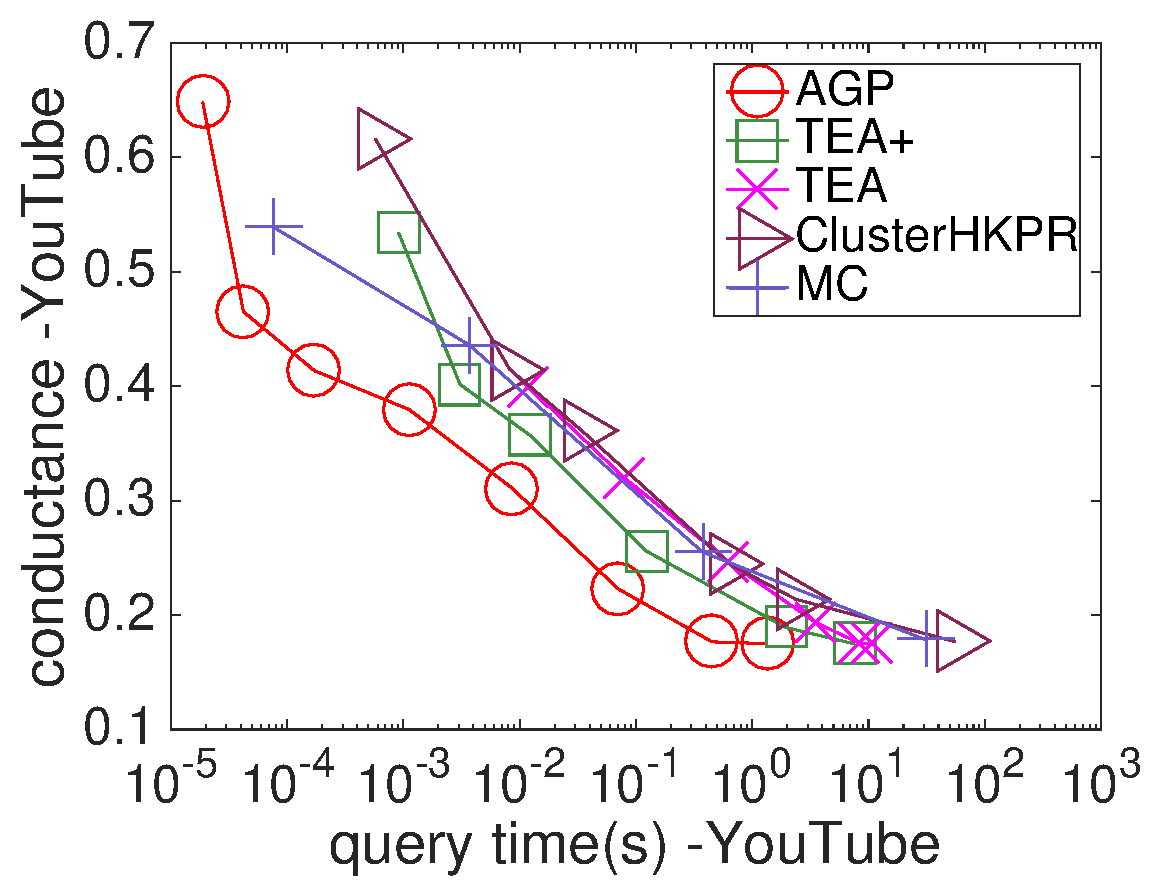
\includegraphics[height=34mm]{./Figs/HKPR-conductance-query-YT.eps} &
%			\hspace{-4mm} 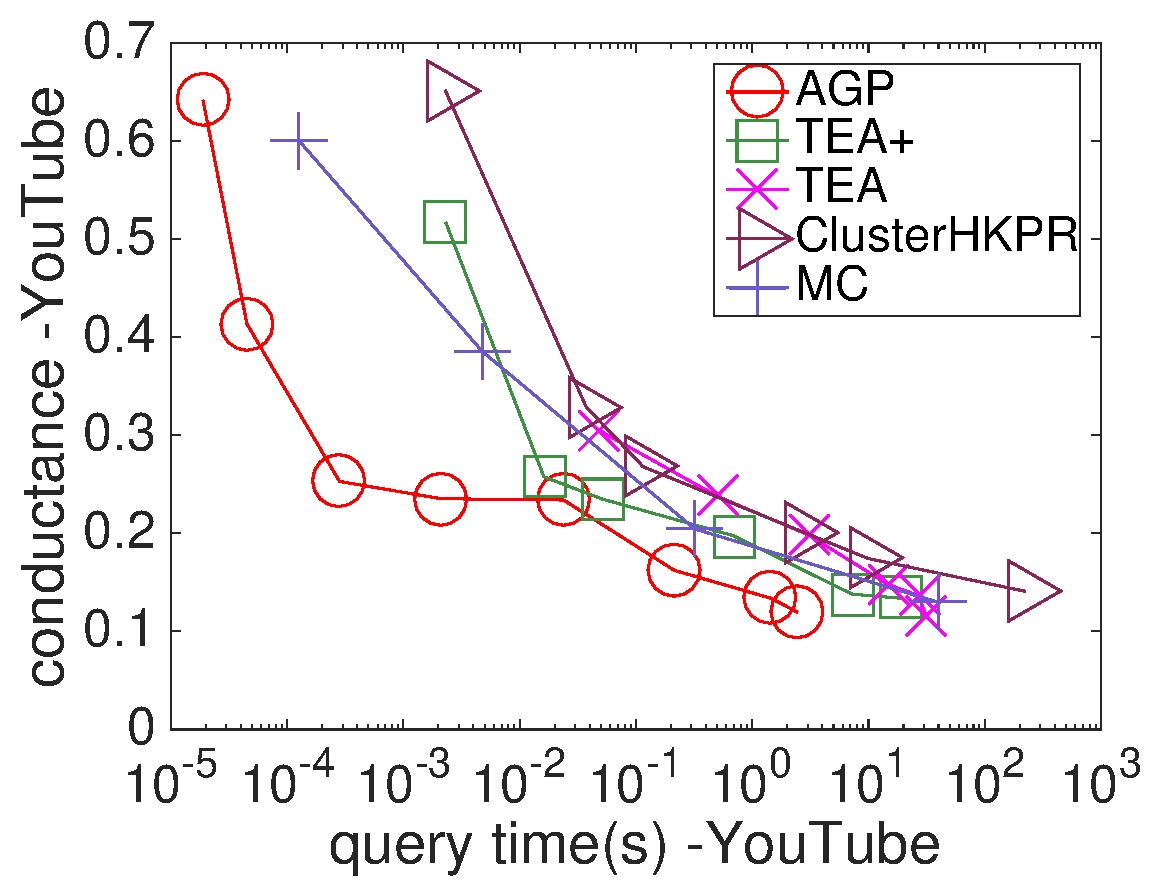
\includegraphics[height=34mm]{./Figs/HKPR-10-conductance-query-YT.eps} &
%			\hspace{-4mm} 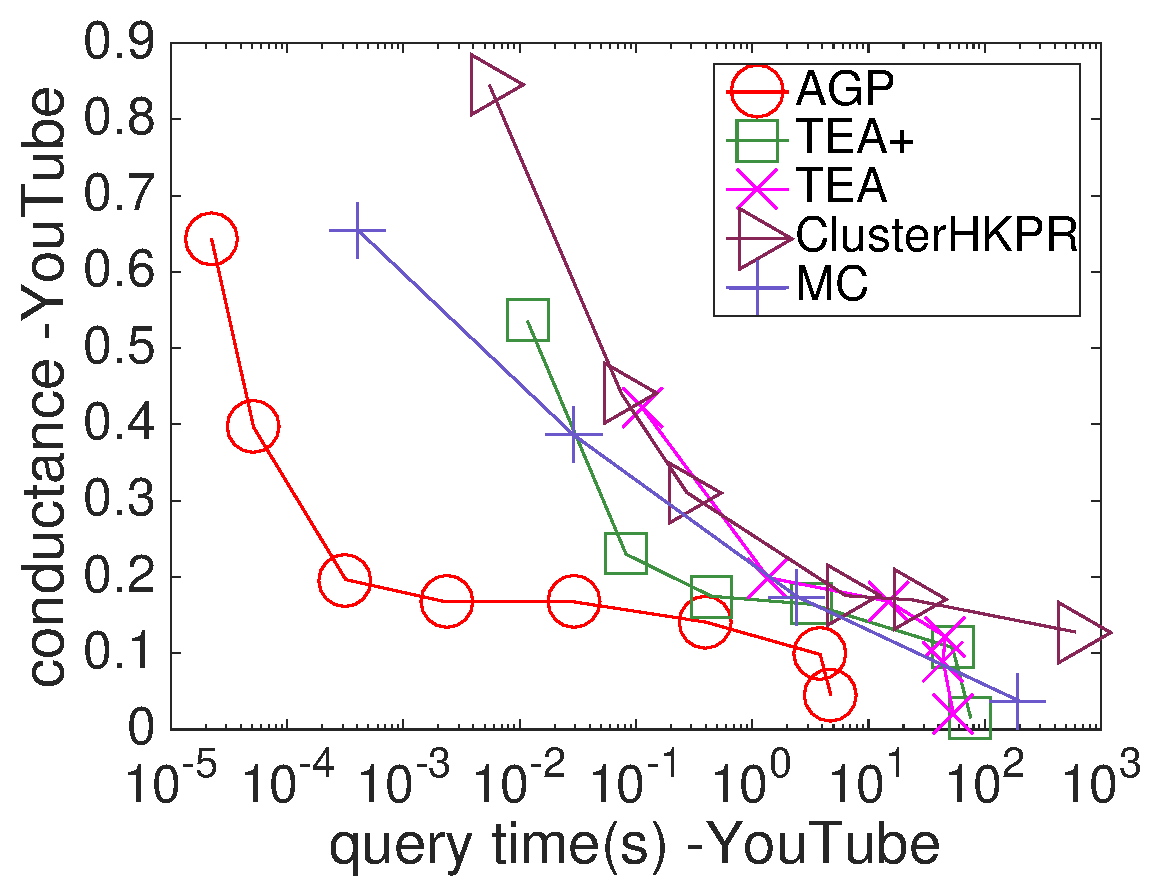
\includegraphics[height=34mm]{./Figs/HKPR-20-conductance-query-YT.eps} &
%			\hspace{-4mm} 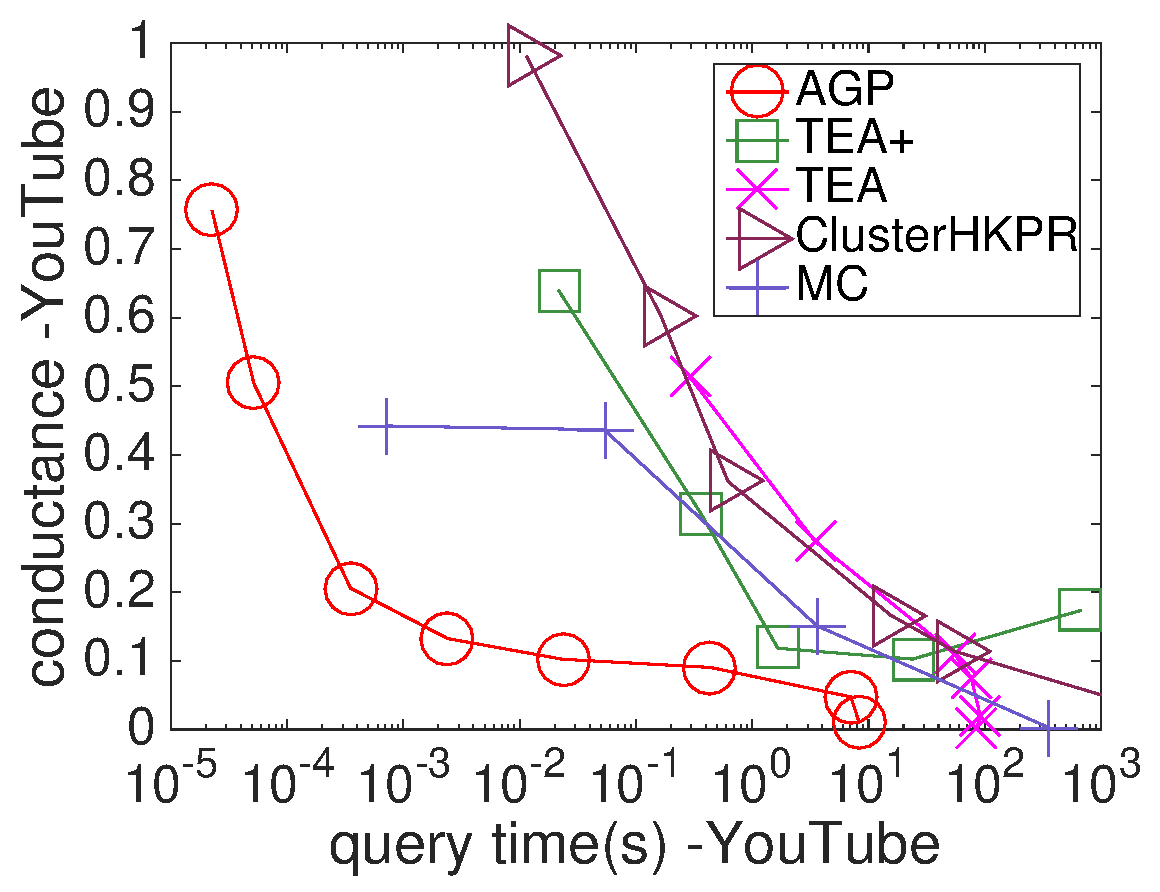
\includegraphics[height=34mm]{./Figs/HKPR-40-conductance-query-YT.eps} \\
%			(a) $t=5$ & (b) $t=10$ & (c) $t=20$ & (d) $t=40$ 
%		\end{tabular}
%		\vspace{-4mm}
%		\caption{Effect of heat constant t for {\em conductance} on {\em Youtube}.}
%		\label{fig:HKPR-conductance-query-YT}
%		\vspace{-2mm}
%	\end{small}
%\end{figure*}



%\begin{figure*}[t]
    %\begin{small}
%		\centering
%		\vspace{-2mm}
		%    \begin{footnotesize}
%		\begin{tabular}{cccc}
%			%\multicolumn{4}{c}{\hspace{-4mm} \includegraphics[height=5mm]{./Figs/legend_large.eps}} \vspace{-1mm} \\
%			\hspace{-2mm} 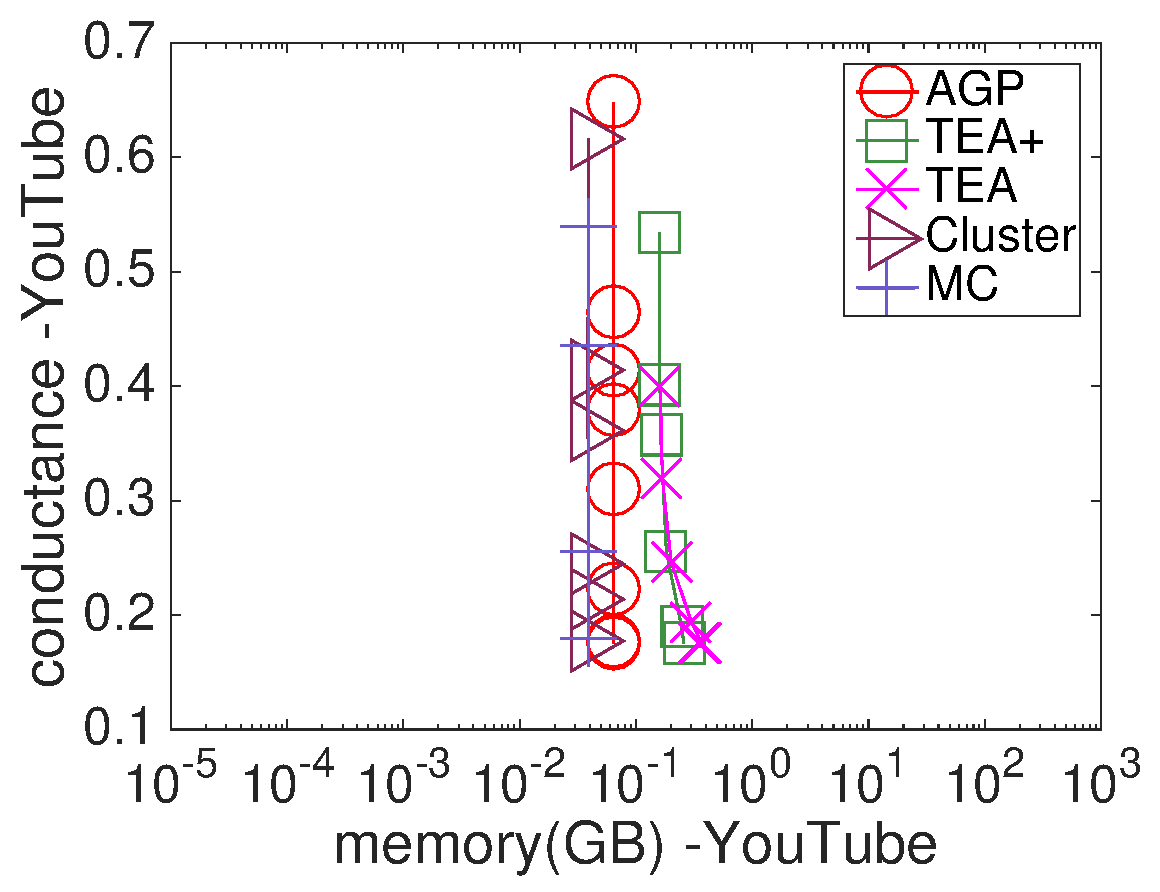
\includegraphics[height=34mm]{./Figs/HKPR-mem-conductance-query-YT_mem.eps} &
%			%\hspace{-3mm} 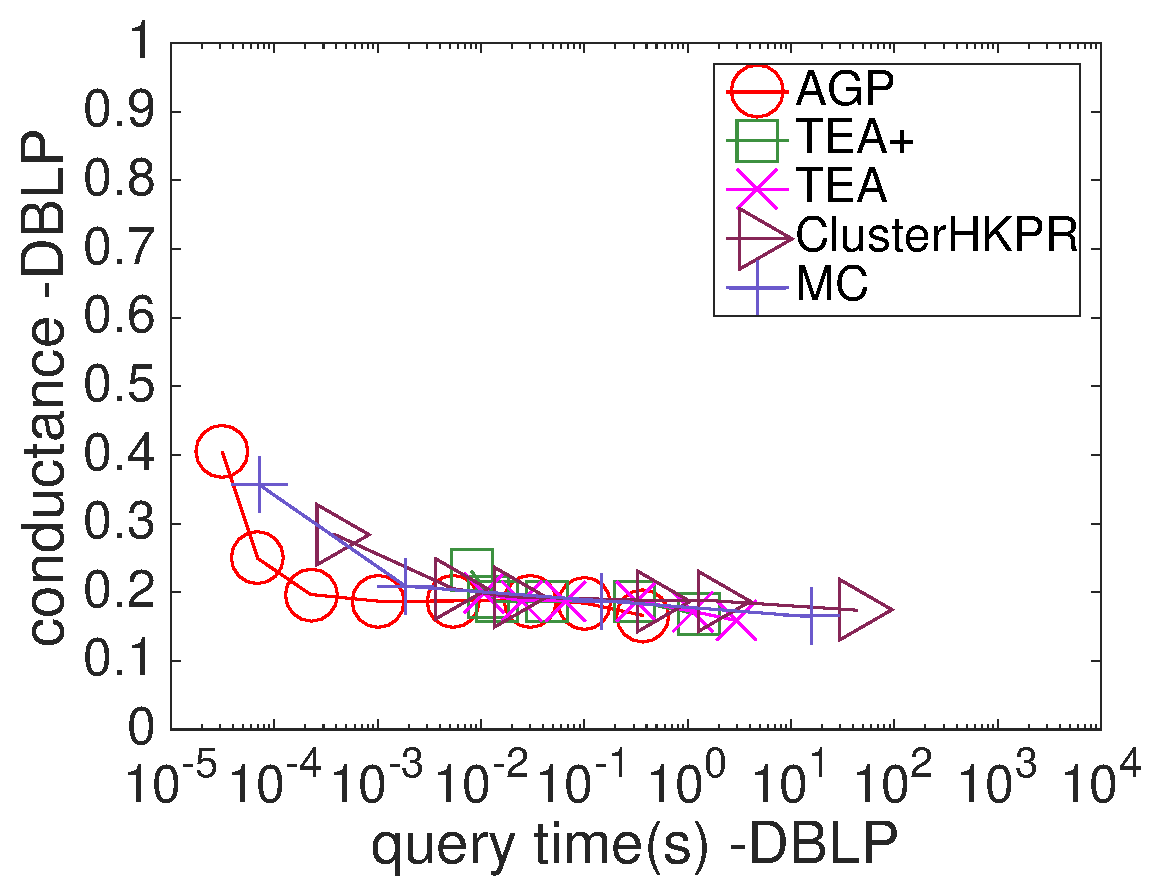
\includegraphics[height=25mm]{./Figs/HKPR-conductance-query-DB.eps} &
%			\hspace{-4mm} 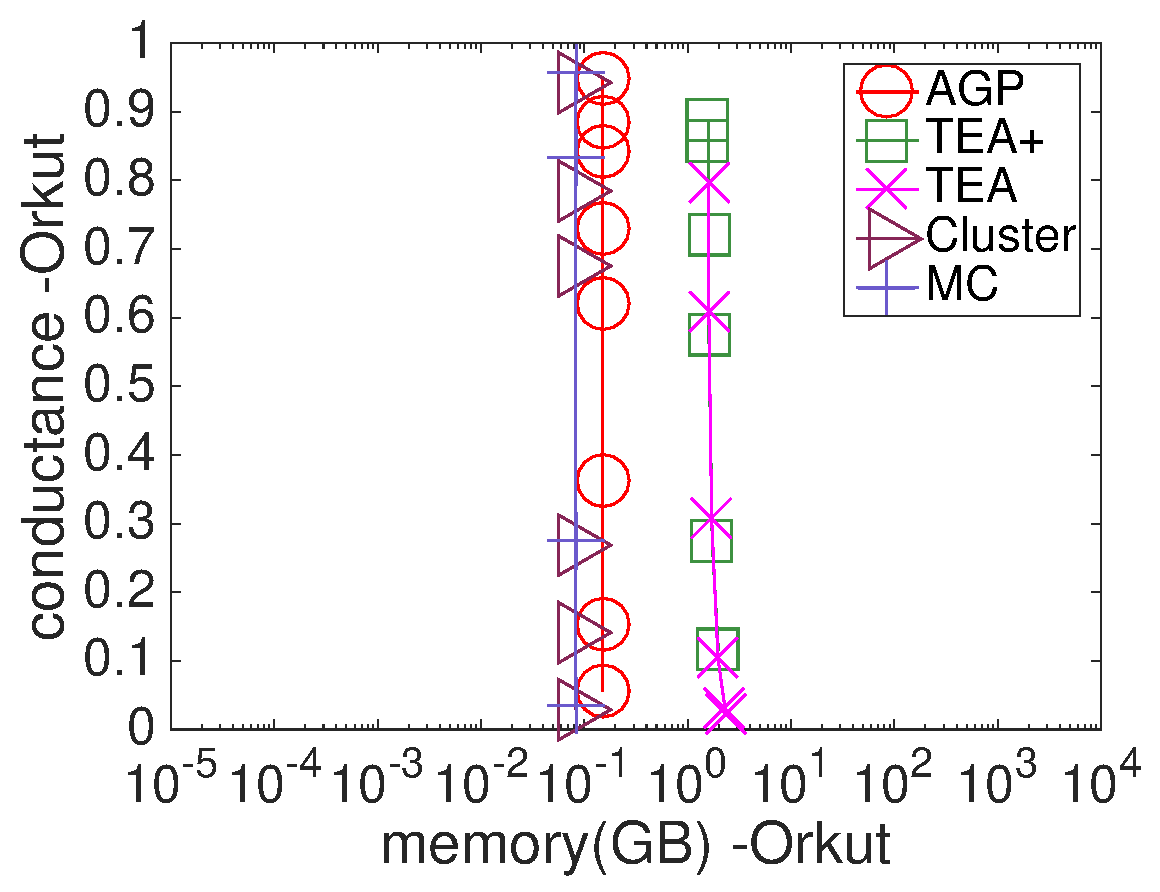
\includegraphics[height=34mm]{./Figs/HKPR-mem-conductance-query-OL_mem.eps} &
%			\hspace{-4mm} 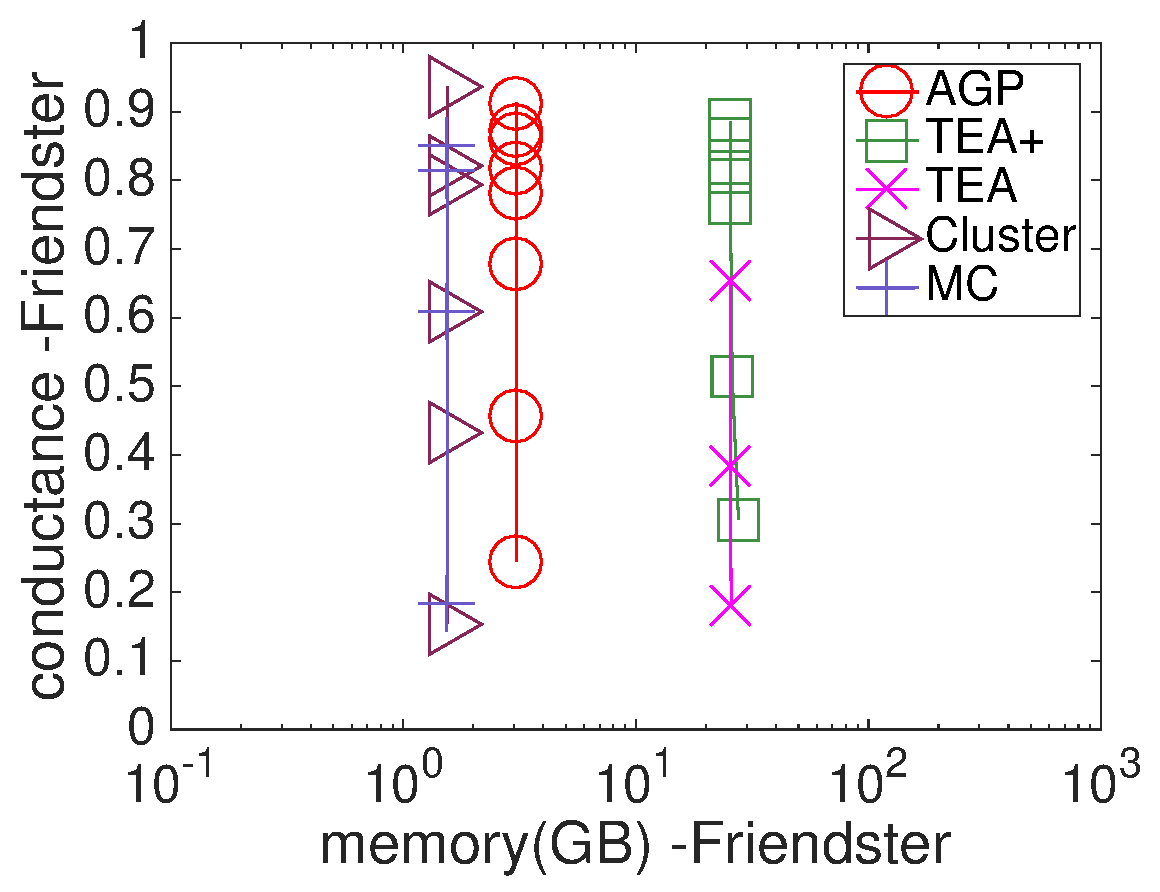
\includegraphics[height=34mm]{./Figs/HKPR-mem-conductance-query-FR_mem.eps} &
%			%\hspace{-4mm} 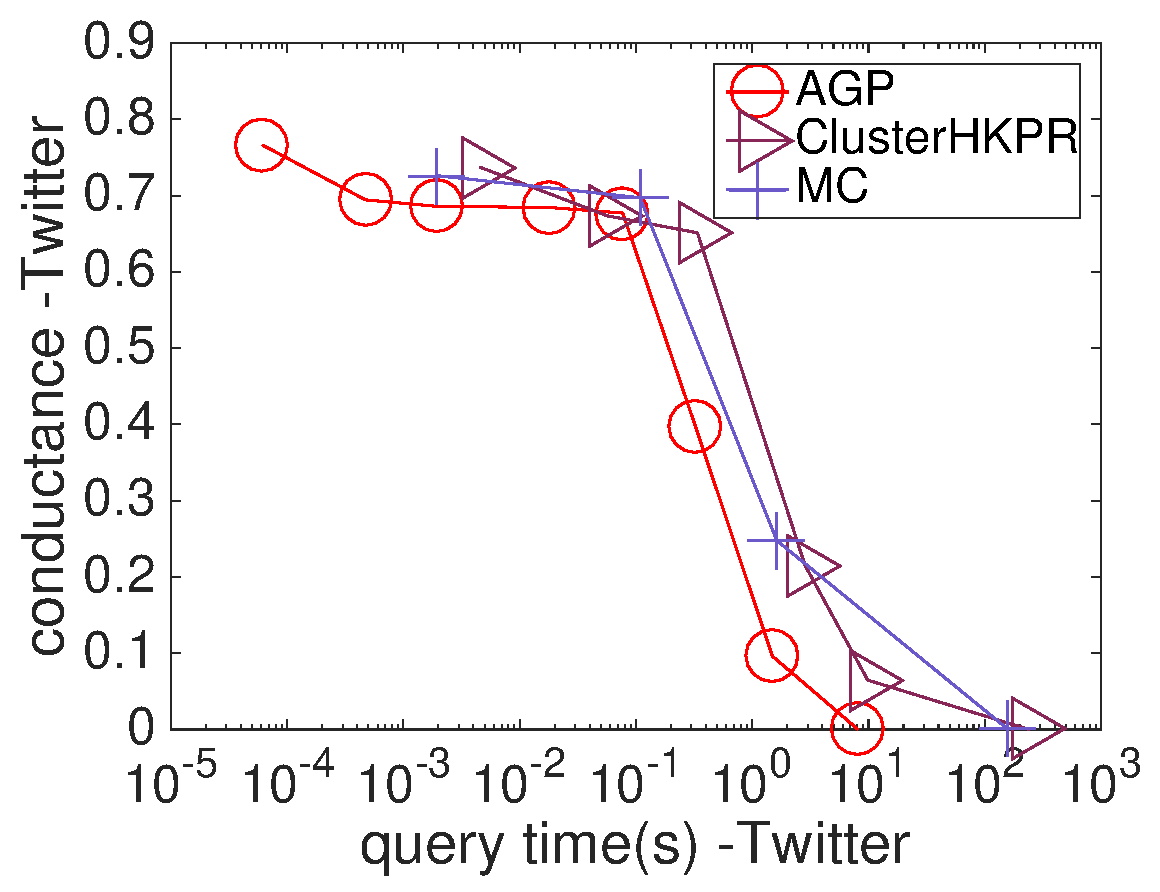
\includegraphics[height=34mm]{./Figs/HKPR-conductance-query-TW.eps} 
%		\end{tabular}
%		\vspace{-4mm}
%		\caption{Tradeoffs between {\em conductance} and overhead memory in local clustering.}
%		\label{fig:HKPR-conductance-mem}
%		\vspace{-2mm}
    %\end{small}
%\end{figure*}



 



%%% Local Variables:
%%% mode: latex
%%% TeX-master: "paper"
%%% End:
